\chapter{并发控制}

\begin{introduction}[期末考试提纲]
  \item X锁、S锁、U锁、IS锁、IX锁、SIX锁
  \item 两段锁协议内容及其作用
  \item 死锁及其解决措施
  \item 基于时间戳的并发控制协议
  \item 基于有效性检查的并发控制协议
  \item MySQL MVCC中的读视图和可见性算法
\end{introduction}

\section{基于锁的协议}

\begin{definition}[封锁]
  \textcolor{red}{封锁}就是一个事务对某个数据对象加锁, 取得对它一定的控制, 限制其它事务对该数据对象使用.
  
  要访问数据项$R$, 事务$T_i$必须先申请对$R$的封锁, 如果$R$已经被事务$T_j$加了不相容的锁, 则$T_i$需要等待, 直至$T_j$释放它的封锁.
\end{definition}

\textcolor{red}{封锁性能}: 事务吞吐量, TPC-C.

\subsection{封锁类型}

\begin{itemize}
  \item 基本锁类型: X锁、S锁、U锁
  \item 意向锁: IS、IX、IU、SIX
  \item 码范围锁: RangeS\_S、RangeI\_N
  \item 其他锁: 模式锁、闩锁、BU锁
\end{itemize}

\begin{definition}[排它锁(X锁, eXclusive lock)]
  lock-X($R$): 又称写锁, 持有X锁可以读写数据项.

  事务$T$对数据对象$R$加上X锁, 则其它事务对$R$的任何封锁请求都
不能成功, 直至$T$释放$R$上的X锁.
\end{definition}

\begin{definition}[共享锁(S锁, Share lock)]
  lock-S($R$): 又称读锁, 持有S
锁只能读取数据项.

事务$T$对数据对象$R$加上X锁, 则其它事务对$R$的任何\textcolor{red}{$X$锁请求}都
不能成功, 而对$R$的S锁请求可以成功.
\end{definition}

封锁的相容矩阵comp(A,B):
\begin{table}[H]
    \centering
    \begin{tabular}{|c|c|c|}
        \hline
        \multirow{2}{*}{\textbf{请求锁模式A}} & \multicolumn{2}{c|}{\textbf{现有锁模式B}} \\ \cline{2-3}
         & \textbf{S} & \textbf{X} \\ \hline
        \textbf{S} & \cellcolor{red!10}\textcolor{blue}{是} & \textcolor{blue}{否} \\ \hline
        \textbf{X} & \textcolor{blue}{否} & \textcolor{blue}{否} \\ \hline
    \end{tabular}
    \caption{封锁的相容矩阵}
    \label{tab:lock_compatibility}
\end{table}

长锁: 保持到事务结束时才释放的锁

短锁: 在事务中途就可以释放的锁

\begin{itemize}
  \item read uncommitted: 不申请锁.
  \item read committed: 短S锁.
  \item repeatable read: 长S锁.
\end{itemize}

\subsection{两阶段封锁协议}

保证可串行化的一种协议是两阶段封锁协议(two-phase Locking protocol). 该协议要求\textbf{每个事务}分两个阶段提出加锁和解锁申请.
\begin{enumerate}
    \item 增长阶段(growing phase): 一个事务可以获得锁, 但不能释放任何锁.
    \item 缩减阶段(shrinking phase): 一个事务可以释放锁, 但不能获得任何新锁.
\end{enumerate}
起初, 一个事务处于增长阶段. 事务根据需要获得锁. 一旦该事务释放了一个锁, 它就进入了缩减阶段, 并且它不能再发出加锁请求.

\begin{definition}[封锁点]
  封锁点: 事务获得其最后封锁的时间.
\end{definition}

\begin{theorem}
  若一组事务均服从两阶段封锁协议, 则它们的调度一定是可串行化的.

  事务调度等价于和其封锁点顺序一致的串行调度.
\end{theorem}

\begin{proof}
  令$\{T_0,T_1,...,T_n\}$是参与调度$S$的事务集. 如果$T_i$对数据项$R$加$A$型锁, $T_j$对数据项$R$加$B$型锁, 且$comp(A,B)=false$. 若$T_i$先于$T_j$, 记作$T_i\to T_j$, 得到一个优先图.

  设$t_i$是$T_i$的封锁点, \textcolor{red}{若$T_i\to T_j$, 则$t_i\to t_j$.}

  若$\{T_0,T_1,...,T_n\}$不可串行化, 则在优先图中存在环, 不妨设为$T_0\to T_1\to \cdots \to T_n \to t_0$, 则$t_0<t_1<\cdots<t_n<t_0$, 矛盾!
\end{proof}

2PL 可以保证调度是可串行化的吗? 可以. 如上.

2PL 可以保证调度是无级联的吗? 不能保证. 在标准的 基本 2PL 中, 一个事务可能读取到另一个尚未提交事务写入的数据(即“脏读”).

\begin{figure}[H]
    \centering
    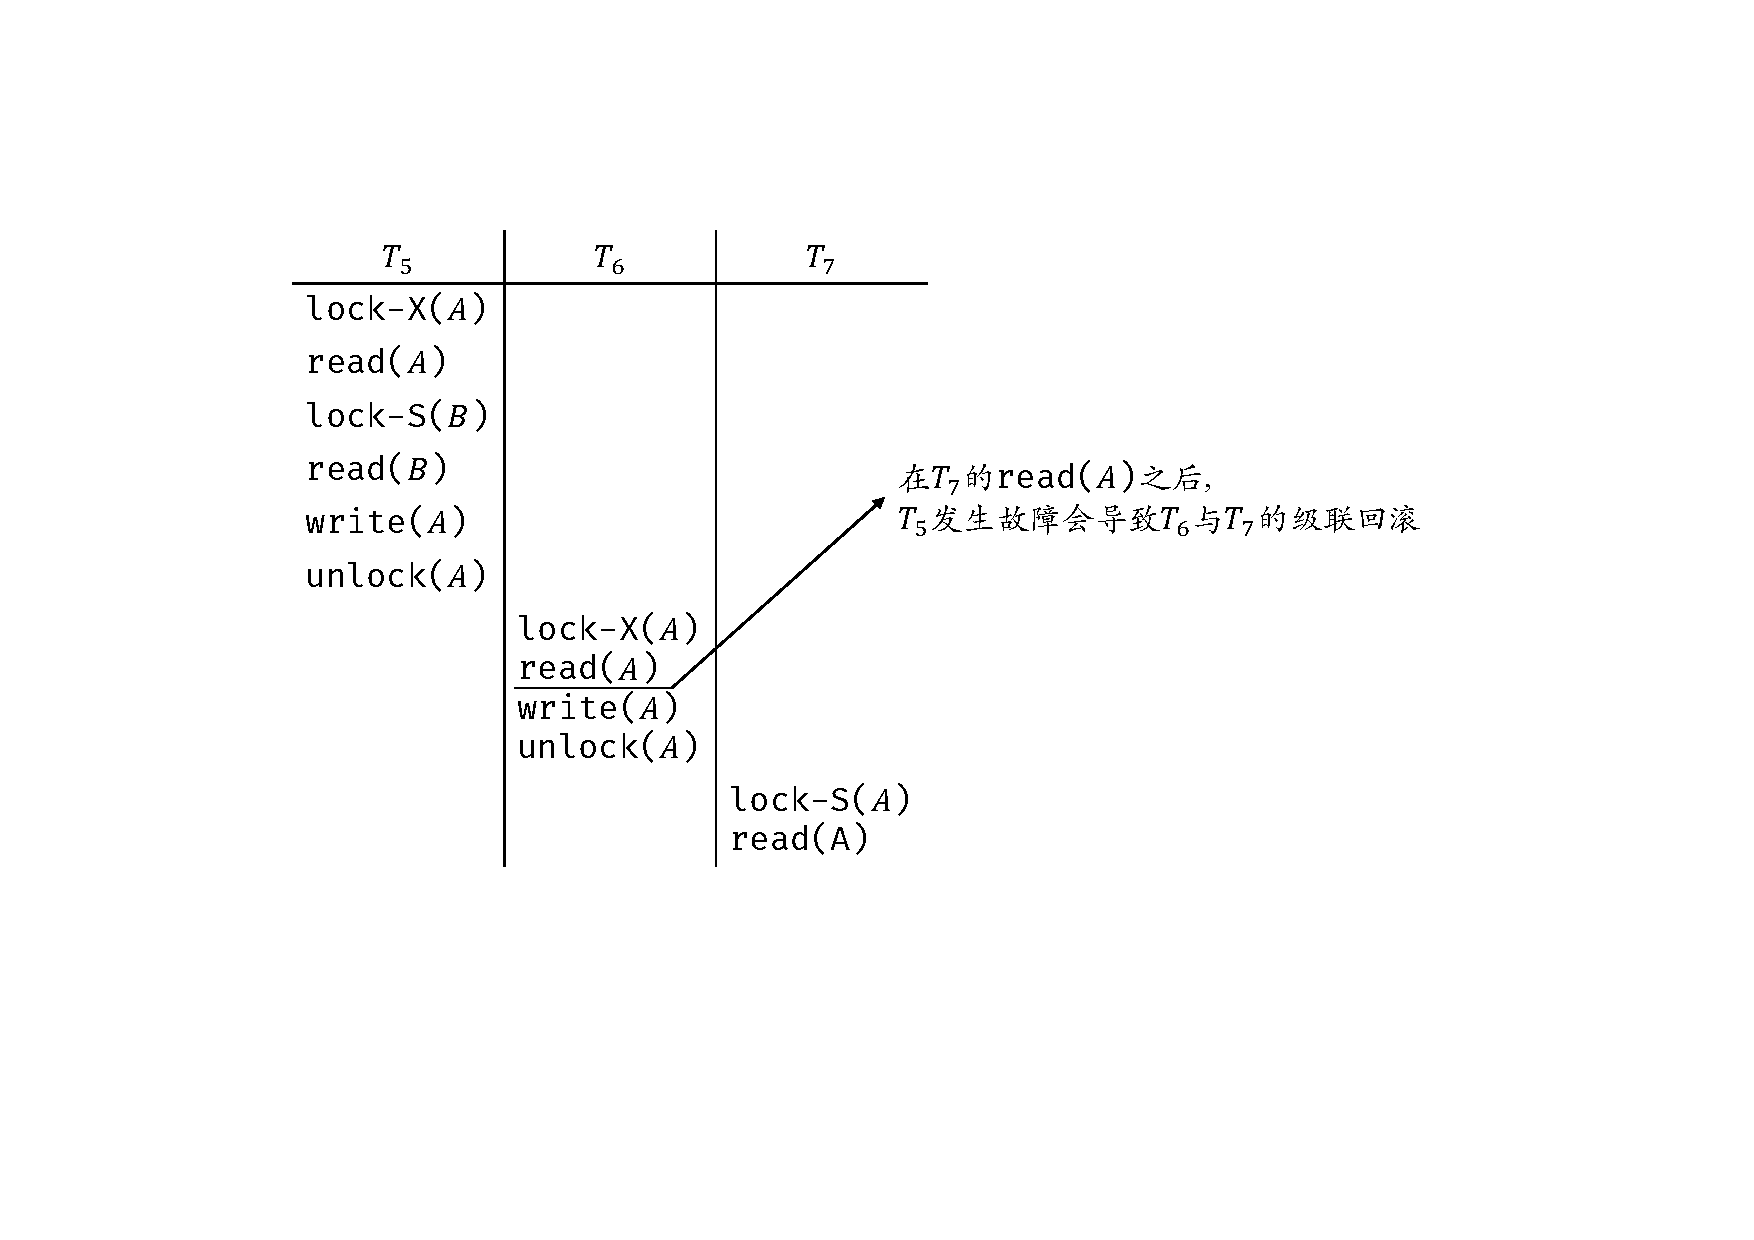
\includegraphics[width=.7\textwidth]{figure/级联.pdf}
    \caption{2PL的级联回滚}
\end{figure}

2PL 可以保证调度避免不可重复读吗? 不一定. 

严格2PL(strict two-phrase locking protocol): 要求X锁是长锁.

严厉2PL(rigorous two-phrase locking protocol): 要求S锁和X锁均是长锁.

\subsection{先读后写: 锁转换}

请考虑下面的两个事务:
\begin{align*}
    &T_1: \text{read}(a_1);\,\text{read}(a_2);...;\text{read}(a_n);\,\text{write}(a_1); \\
    &T_2: \text{read}(a_1);\,\text{read}(a_2);\text{display}(a_1+a_2);
\end{align*}

如果我们采用两阶段封锁协议, 则$T_1$必须以排他模式封锁$a_1$. 此时, 两个事务的任何并发执行都相当于一个串行执行. 所以, 我们可以在开始时以共享模式封锁$a_1$, 随后把这个锁变更为排他锁.

上面介绍的就是\textbf{锁转换(lock conversion)}:
\begin{enumerate}
    \item 升级(upgrade): 从共享到排他的转换;
    \item 降级(downgrade): 从排他到共享的转换.
    \item 升级只能发生在增长阶段, 而降级只能发生在缩减阶段。
\end{enumerate}

\begin{problem}
  升级锁和重新申请锁有区别吗?
\end{problem}

\begin{itemize}
  \item 排队顺序不同
  \item 升级锁已经在队列中, 可以更快获得批准; 重新申请锁需要从头排队, 获取锁更慢.
\end{itemize}

\begin{problem}
  在哪个隔离性级别下会出现锁转换?
\end{problem}
\begin{itemize}
  \item repeated committed 以及更高的隔离级别
  \item Read committed 和 read uncommitted 不出现锁转换, 因为锁转换要求一直持有读锁, 没有释放.
\end{itemize}

但是锁转换会带来死锁的问题: 
\begin{figure}[H]
    \centering
    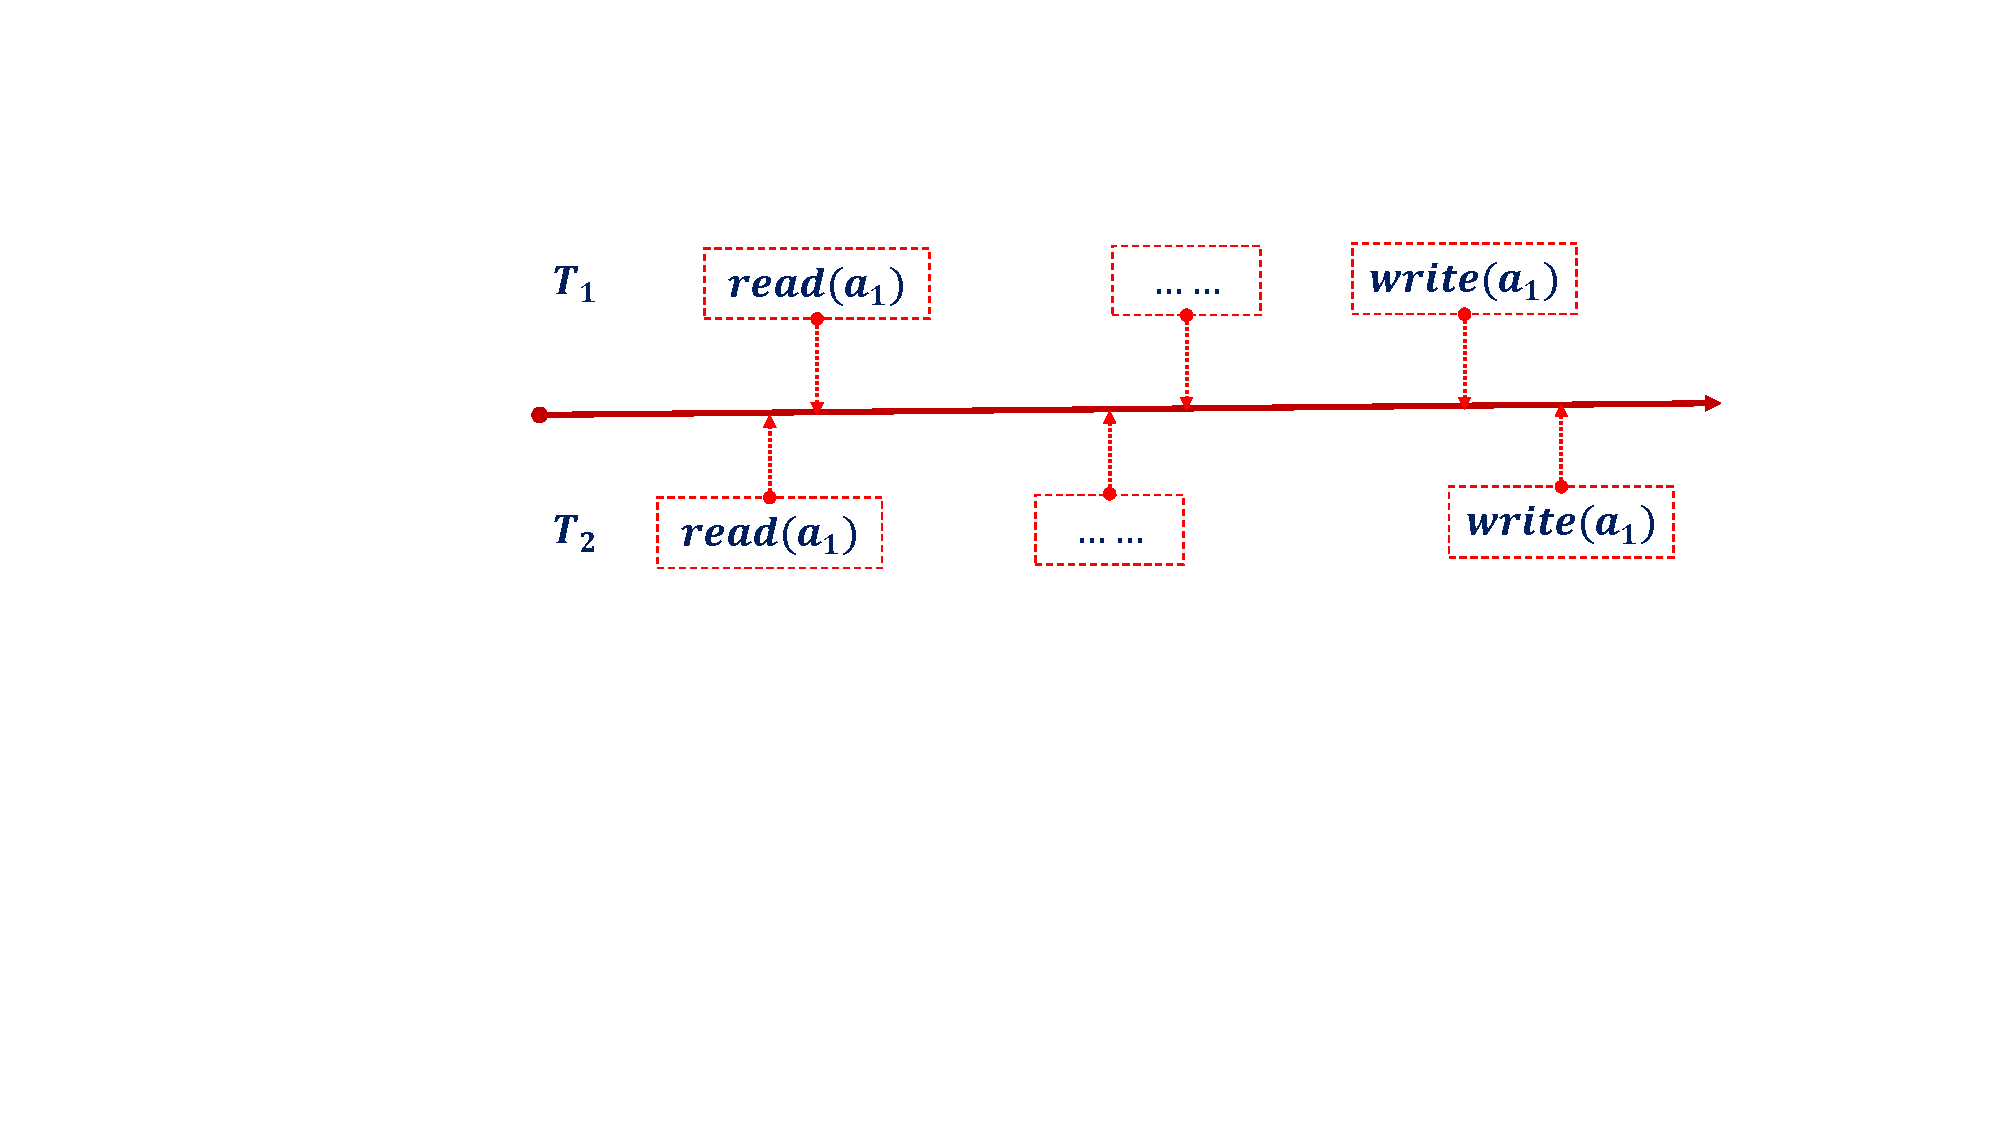
\includegraphics[width=.6\textwidth]{figure/并发控制-锁转换.pdf}
    \caption{转换死锁}
\end{figure}

如果都使用升级锁: T1要升级锁的时候, 会被T2的读锁阻止; T2要升级锁的时候, 会被T1的读锁阻止


\subsection{先读后写: 更新锁}

\begin{definition}[更新锁(U锁, Update lock)]
  当一个事务查询数据以便将来要进行修改时, 可以对数据项施加更新锁. (\textcolor{red}{这是一种相容性介于S锁和X锁之间的锁.})

  如果事务修改资源, 需将更新锁转换为排它锁.

  一次只有一个事务可以获得资源上的更新锁.
\end{definition}

此时的相容矩阵comp(A,B):
\begin{table}[H]
    \centering
    \begin{tabular}{|c|c|c|c|}
        \hline
        \multirow{2}{*}{\textbf{请求锁模式A}} & \multicolumn{3}{c|}{\textbf{现有锁模式B}} \\ \cline{2-4}
         & \textbf{S} & \textbf{X} & \textbf{U} \\ \hline
        \textbf{S} & \textcolor{blue}{是} & \textcolor{blue}{否} & \textcolor{blue}{是} \\ \hline
        \textbf{X} & \textcolor{blue}{否} & \textcolor{blue}{否} & \textcolor{blue}{否} \\ \hline
        \textbf{U} & \cellcolor{red!10}\textcolor{blue}{是} & \textcolor{blue}{否} & \cellcolor{red!10}\textcolor{blue}{否} \\ \hline
    \end{tabular}
    \caption{封锁的相容矩阵}
\end{table}

\subsection{封锁粒度}

封锁对象:属性值、元组、关系、数据库、索引项、索引、物理页、块

\begin{itemize}
  \item 封锁粒度大: 锁的数目少, 开销小; 冲突几率大, 并发度低
  \item 封锁粒度小: 锁的数目多, 开销大; 冲突几率小, 并发度高
\end{itemize}

\begin{definition}[事务的完整性相关域]
  事务的完整性相关域: 只封锁与操作有关的的数据对象.
\end{definition}

但是问题出现了: 比如对整个表的封锁会和对行的封锁之间产生冲突!

\textcolor{red}{如何检测到不同粒度之间的锁的隐含冲突?}

如果有事务T1对某元组加了S锁, 而事务T2对该元组所在的关系加了X锁, 实则隐含地X封锁了该元组, 从而造成矛盾.

\begin{definition}[意向锁(I锁, Intend lock)]
  当为某节点加上I锁, 表明其某些内层节点已发生事实上的封锁, 防止其它事务再去显式封锁该节点. 表示它的后裔节点拟进行封锁.

  从封锁层次的根开始实施I锁, 依次占据路径上的所有节点, 直至要真正进行显式封锁的节点的父节点为止.
\end{definition}

此时的相容矩阵comp(A,B):
\begin{table}[H]
    \centering
    \begin{tabular}{|c|c|c|c|}
        \hline
        \multirow{2}{*}{\textbf{请求锁模式A}} & \multicolumn{3}{c|}{\textbf{现有锁模式B}} \\ \cline{2-4}
         & \textbf{I} & \textbf{X} & \textbf{S} \\ \hline
        \textbf{I} & \cellcolor{red!10}\textcolor{blue}{是} & \textcolor{blue}{否} & \textcolor{blue}{否} \\ \hline
        \textbf{X} & \textcolor{blue}{否} & \textcolor{blue}{否} & \textcolor{blue}{否} \\ \hline
        \textbf{S} & \textcolor{blue}{否} & \textcolor{blue}{否} & \textcolor{blue}{是} \\ \hline
    \end{tabular}
    \caption{封锁的相容矩阵}
\end{table}

\begin{figure}[H]
    \centering
    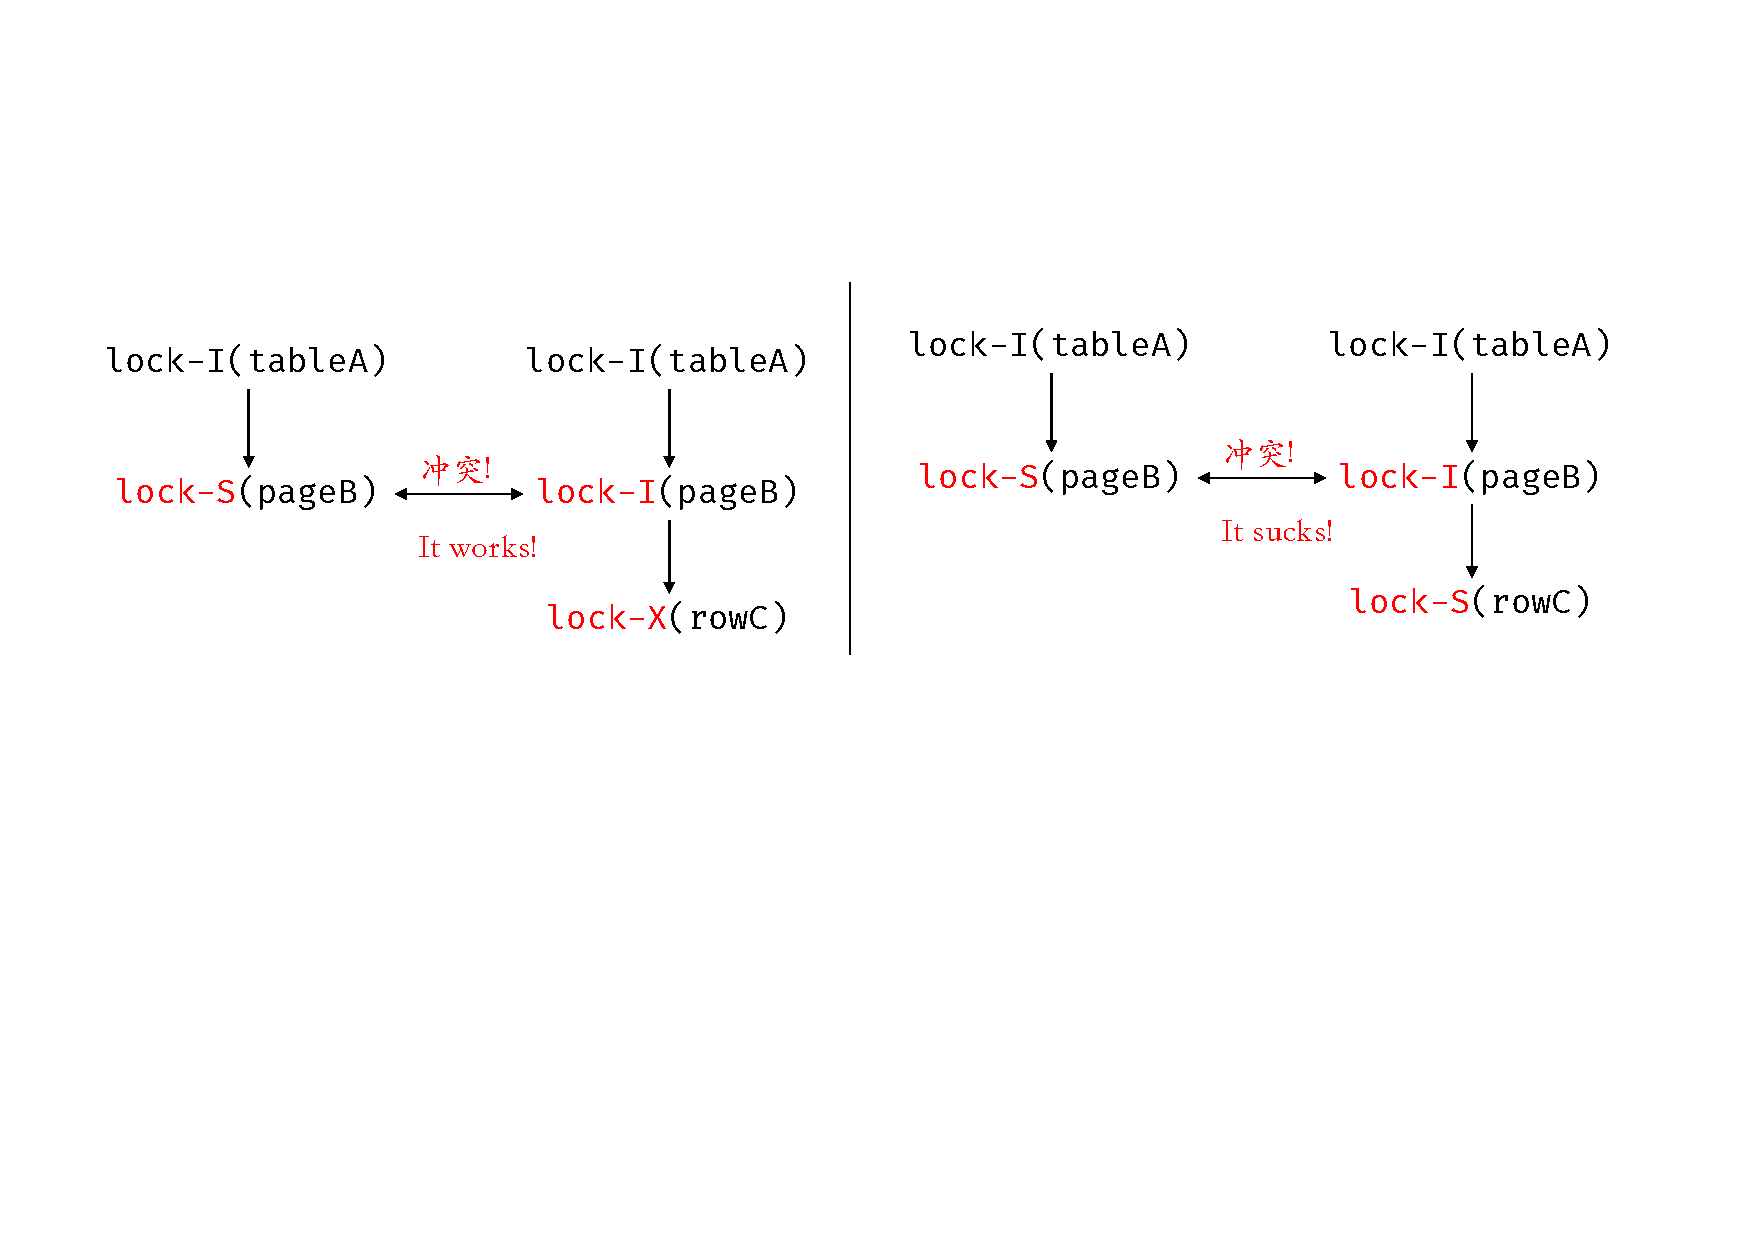
\includegraphics[width=.8\textwidth]{figure/I锁冲突.pdf}
    \caption{意向锁I的不足之处}
\end{figure}

I锁没有揭示内层锁的性质.

\begin{definition}[IS锁]
  对一个数据对象加IS锁, 表示它的后裔节点拟(意向)加S锁.
\end{definition}

\begin{definition}[IX锁]
  对一个数据对象加IX锁, 表示它的后裔节点拟(意向)加X锁.
\end{definition}

此时的相容矩阵comp(A,B):
\begin{table}[H]
    \centering
    \begin{tabular}{|c|c|c|c|c|}
        \hline
        \multirow{2}{*}{\textbf{请求锁模式A}} & \multicolumn{4}{c|}{\textbf{现有锁模式B}} \\ \cline{2-5}
         & \textbf{IS} & \textbf{S} & \textbf{IX} & \textbf{X} \\ \hline
        \textbf{IS} & \textcolor{blue}{是} & \cellcolor{red!10}\textcolor{blue}{是} & \textcolor{blue}{是} & \textcolor{blue}{否} \\ \hline
        \textbf{S} & \textcolor{blue}{是} & \textcolor{blue}{是} & \cellcolor{red!10}\textcolor{blue}{否} & \textcolor{blue}{否} \\ \hline
        \textbf{IX} & \textcolor{blue}{是} & \textcolor{blue}{否} & \cellcolor{red!10}\textcolor{blue}{是} & \textcolor{blue}{否} \\ \hline
        \textbf{X} & \textcolor{blue}{否} & \textcolor{blue}{否} & \textcolor{blue}{否} & \textcolor{blue}{否} \\ \hline
    \end{tabular}
    \caption{封锁的相容矩阵}
\end{table}

\begin{figure}[H]
    \centering
    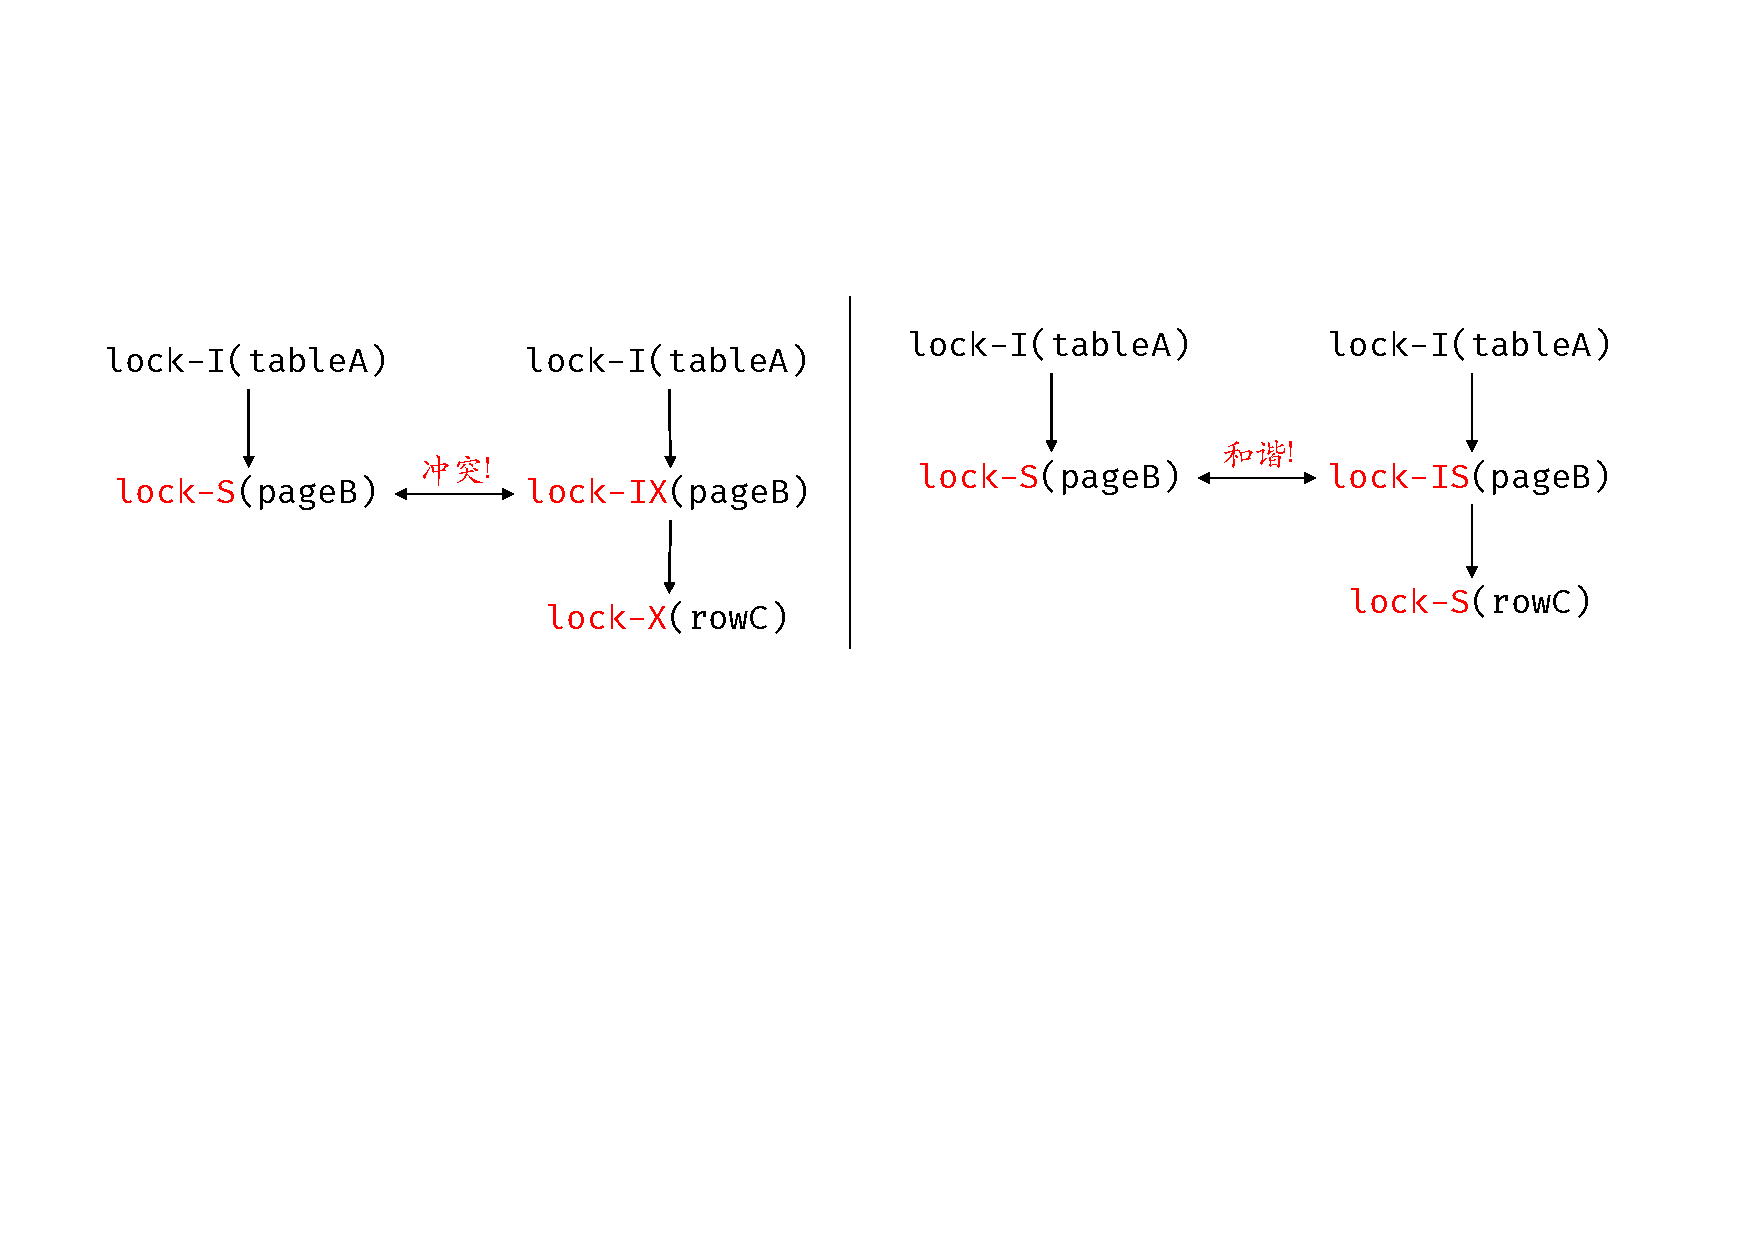
\includegraphics[width=.8\textwidth]{figure/意向锁-和谐.pdf}
    \caption{意向锁I的细化}
\end{figure}

SIX = S + IX: 对表加SIX锁, 表示该事务要读整个表(S锁), 同时会更新个别元组(IX锁).

此时的相容矩阵comp(A,B):
\begin{table}[H]
    \centering
    \begin{tabular}{|c|c|c|c|c|c|c|}
        \hline
        \multirow{2}{*}{\textbf{请求锁模式A}} & \multicolumn{6}{c|}{\textbf{现有锁模式B}} \\ \cline{2-7}
         & \textbf{IS} & \textbf{S} & \textbf{U} & \textbf{IX} & \textbf{SIX} & \textbf{X} \\ \hline
        \textbf{IS}  & 是 & 是 & 是 & 是 & \textcolor{red}{是} & 否 \\ \hline
        \textbf{S}   & 是 & 是 & 是 & 否 & 否 & 否 \\ \hline
        \textbf{U}   & 是 & 是 & 否 & 否 & 否 & 否 \\ \hline
        \textbf{IX}  & 是 & 否 & 否 & 是 & 否 & 否 \\ \hline
        \textbf{SIX} & 是 & 否 & 否 & 否 & 否 & 否 \\ \hline
        \textbf{X}   & 否 & 否 & 否 & 否 & 否 & 否 \\ \hline
    \end{tabular}
    \caption{封锁的相容矩阵}
\end{table}

\subsection{码范围锁}

\begin{lstlisting}[language=SQL, caption={幻象例子}]
-- 事务 T1:
SELECT * FROM student WHERE score > 90;  -- 返回张三
-- 事务 T2:
INSERT INTO student VALUES ('李四', 95); -- 成功
-- T1 再次执行:
SELECT * FROM student WHERE score > 90;  -- 返回张三和李四,幻读发生
\end{lstlisting}

对于 \verb|select * from R where A >=10 and A <=20|, 在两次读取之间可能出现幻象(也就是两次读取之间出现了插入, 导致满足条件的元组发生了改变).
\begin{itemize}
  \item 此时单纯封锁现有数据是无效的. 如何防止其他事务往区间[10, 20]插入数据?
  \item 一种解决思路: 封锁整个表. \textit{并发度极低!}
  \item 第二种解决思路: 码范围锁. \textcolor{red}{条件: 查询/操作字段上必须有合适的索引; 当前事务隔离级别为: REPEATABLE READ / SERIALIZABLE.}
\end{itemize}

码范围锁通过\textcolor{red}{覆盖索引行和索引行之间的范围}来工作, 因为第二个事务在
该范围内进行任何行插入、更新或删除操作时均需要修改索引, 而码范围
锁覆盖了索引项, 所以在第一个事务完成之前会阻塞第二个事务的进行.

码范围锁包括:
\begin{itemize}
  \item \textcolor{red}{范围组件}. 表示保护两个连续索引项之间范围的锁模式(RangeT).
  \item \textcolor{red}{行组件}. 表示保护索引项的锁模式(K).
  \item 把这两部分用下划线连接, 如RangeT\_K.
\end{itemize}

\begin{lstlisting}[language=SQL, caption={码范围锁典型触发示例}]
-- 满足所有触发条件的例子:
BEGIN;

SELECT * FROM student 
WHERE score > 90 
FOR UPDATE;  -- 或 LOCK IN SHARE MODE

-- 使用的是InnoDB引擎、字段有索引、使用范围条件、隔离级别为RR或更高
\end{lstlisting}

此时会触发 Next-Key Lock (即 Key-Range Lock), 锁定:
\begin{itemize}
  \item 现有符合条件的记录
  \item 它们前后的间隙
  \item 插入位置(防止幻读)
\end{itemize}


\begin{table}[H]
\centering
\begin{tabular}{|c|c|c|c|}
  \hline
\textbf{范围} & \textbf{行} & \textbf{模式} & \textbf{描述} \\
\hline
RangeS & S & RangeS\_S & 共享范围, 共享资源锁; 可串行范围扫描 \\
\hline
RangeS & U & RangeS\_U & 共享范围, 更新资源锁; 可串行更新扫描 \\
\hline
RangeI & NULL & RangeI\_N & 插入范围, 空资源锁; 用于在索引中插入新码之前测试范围 \\
\hline
RangeX & X & RangeX\_X & 排它范围, 排它资源锁; 用于更新范围中的码 \\
\hline
\end{tabular}
\caption{码范围锁模式(SQL Server)}
\end{table}



\begin{table}[H]
    \centering
    \begin{tabular}{|c|c|c|c|c|c|c|c|}
        \hline
        \multirow{2}{*}{\textbf{\textcolor{blue}{请求模式}}} & \multicolumn{7}{c|}{\textbf{\textcolor{blue}{现有的授权模式}}} \\ \cline{2-8}
         & \textcolor{red}{\textbf{S}} & \textcolor{red}{\textbf{U}} & \textcolor{red}{\textbf{X}} 
         & \textcolor{red}{\textbf{RangeS\_S}} & \textcolor{red}{\textbf{RangeS\_U}} 
         & \textcolor{red}{\textbf{RangeI\_N}} & \textcolor{red}{\textbf{RangeX\_X}} \\ \hline
         
        \textcolor{red}{共享 (S)} & 是 & 是 & 否 & 是 & 是 & 是 & 否 \\ \hline
        \textcolor{red}{更新 (U)} & 是 & 否 & 否 & 是 & 否 & 是 & 否 \\ \hline
        \textcolor{red}{排它 (X)} & 否 & 否 & 否 & 否 & 否 & 是 & 否 \\ \hline

        \rowcolor{lightred}
        \textcolor{red}{RangeS\_S} & 是 & 是 & 否 & 是 & 是 & 否 & 否 \\ \hline
        \rowcolor{lightred}
        \textcolor{red}{RangeS\_U} & 是 & 否 & 否 & 是 & 否 & 否 & 否 \\ \hline
        \rowcolor{lightred}
        \textcolor{red}{RangeI\_N} & \textcolor{red}{是} & 是 & \textcolor{red}{是} & \textcolor{red}{否} & 否 & 是 & 否 \\ \hline
        \rowcolor{lightred}
        \textcolor{red}{RangeX\_X} & 否 & 否 & 否 & 否 & 否 & 否 & 否 \\ \hline
    \end{tabular}
    \caption{码范围锁的相容矩阵}
\end{table}

码范围锁实际上就是: 1. 对表里这个范围上锁, 2. 对这个表的索引上锁.

现在考虑下面的查询:
\begin{lstlisting}[language=SQL]
select *
from employees
where last_name between 'Delaney' and 'DuLaney'
\end{lstlisting}

根据下面的这个表的索引\ref{fig:key-range}, 我们知道, 实际上读到的是: Dallas, Donovan, Duluth.

为了防止幻读, 数据库会在范围两侧的区间加码范围锁: 加 RangeS\_S 锁在
\begin{itemize}
  \item 区间1: (Dallas, Donovan]
  \item 区间2: (Donovan, Duluth]
\end{itemize}

此时其他事务无法插入 Dashagua, 因为 Dashagua 位于 (Dallas, Donovan] 之间.

\begin{figure}[H]
    \centering
    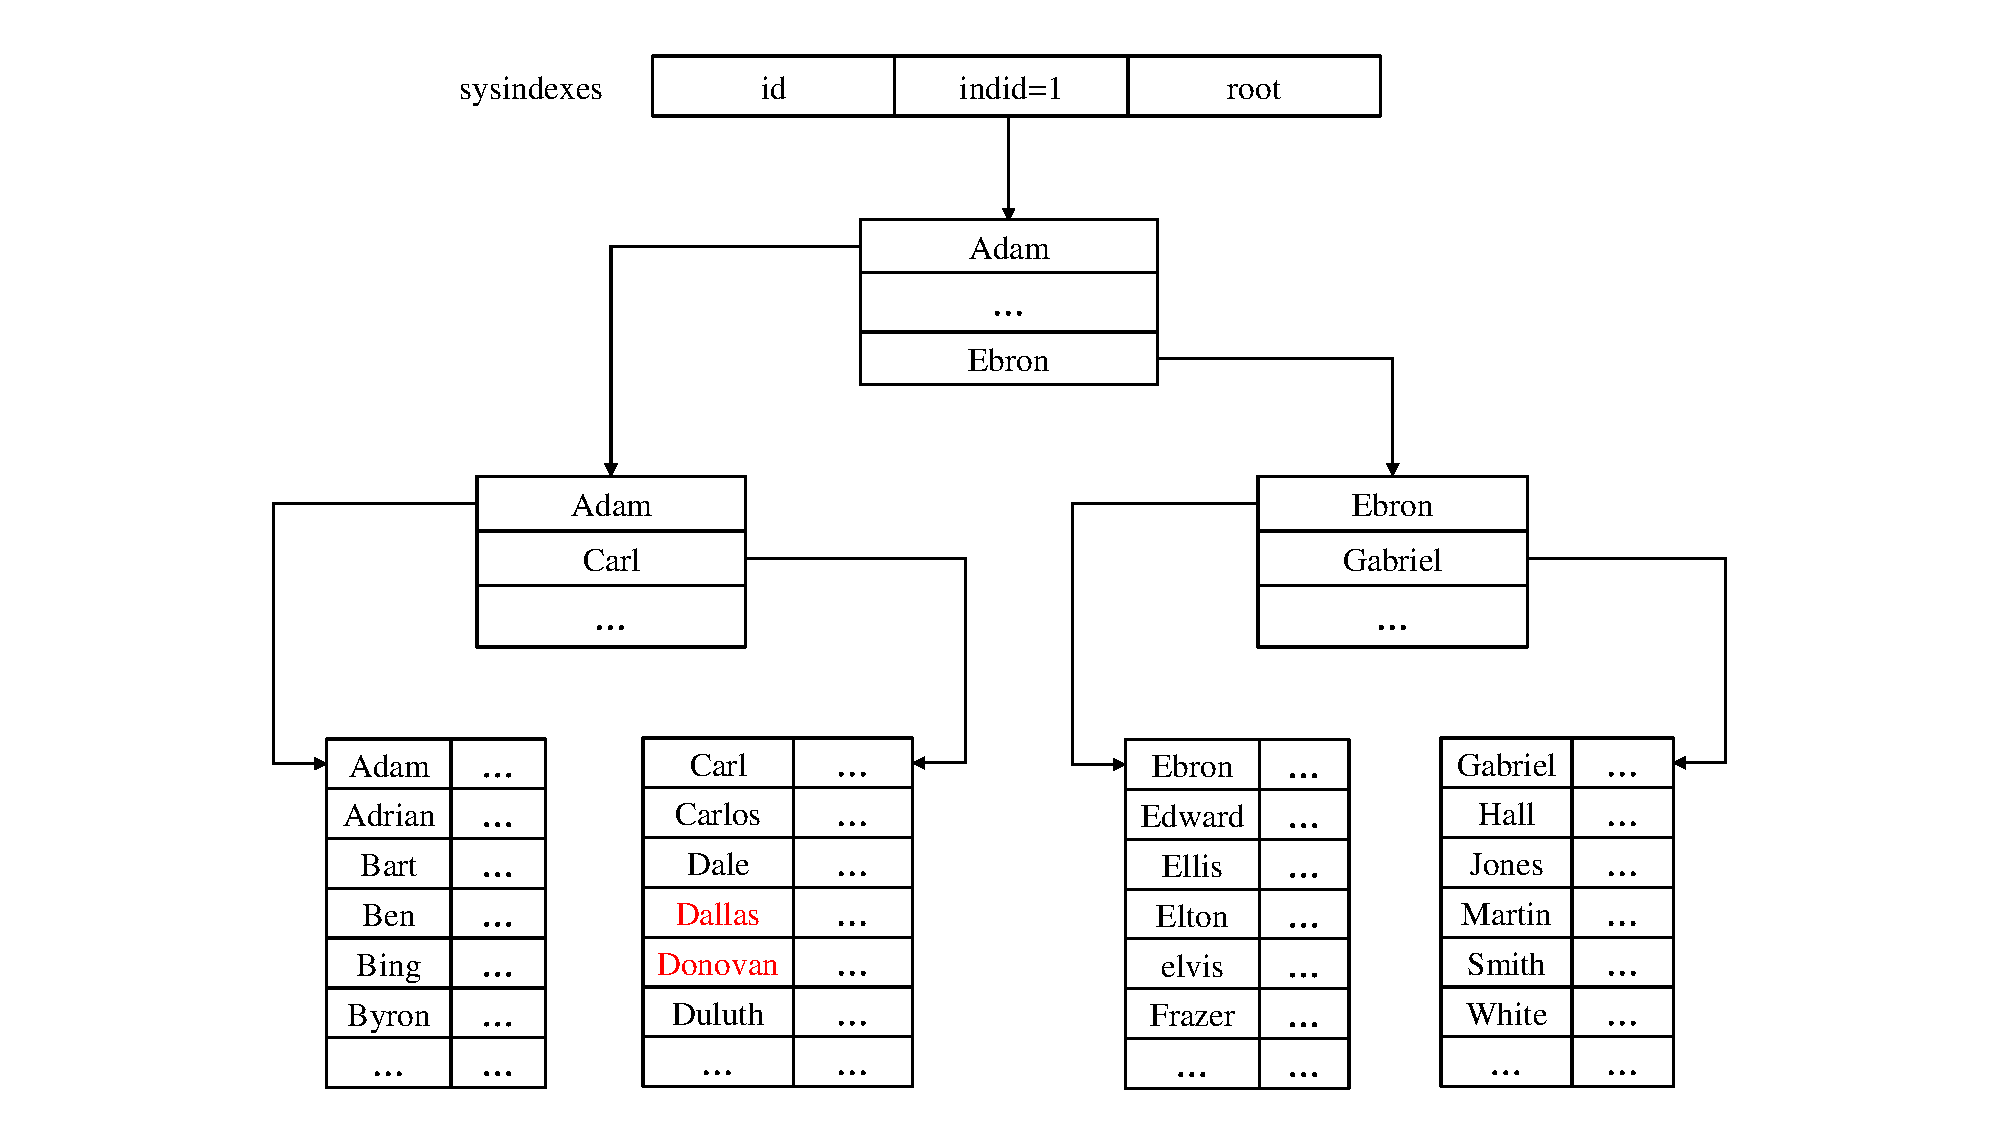
\includegraphics[width=.9\textwidth]{figure/码范围锁.pdf}
    \caption{码范围锁示例}
    \label{fig:key-range}
\end{figure}

\subsection{一些具体系统中的特殊锁模式}

\begin{itemize}
  \item 闩锁
  \item SQL Server的锁模式
  \item MySQL的锁模式
\end{itemize}

Latch(闩锁)是数据库系统和操作系统中用于短时间内保护关键资源的一种轻量级同步机制. 
用于保护数据库内部结构(如缓存页、索引节点等)的并发访问, 通常持续时间非常短.

在 SQL Server 中, 模式锁(Schema Lock)是一种特殊的锁类型, 用于保护数据库对象的结构(shema), 例如表结构、索引、存储过程等, 它防止其他会话对正在变更结构的对象做冲突操作, 确保元数据的一致性.
\begin{itemize}
  \item 模式修改锁(Schema Modification, Sch-M): 改结构时获取, 互斥;
  \item 模式稳定锁(Schema Stability, Sch-S): 读结构时获取, 允许并发.
\end{itemize}

MySQL中的行锁模式: MySQL的行锁只出现在基于索引的查找中.
\begin{itemize}
  \item lock\_rec\_not\_gap(记录锁, 不包含间隙): 只锁定具体的索引记录(行), 不锁定它前后的间隙. \textit{适用于 READ COMMITTED 隔离级别时的普通行锁.}
  \item lock\_gap(间隙锁): 锁定两个索引记录之间的间隙, 不锁定具体的记录. $\to$ 避免幻读. \textit{在可重复读(REPEATABLE READ)隔离级别中常见.}
  \item lock\_ordinary(普通锁, 也叫 Next-Key Lock): 锁定一个具体的记录及其前面的间隙, 是 InnoDB 默认使用的行锁类型.
  \item lock\_insert\_intention(插入意向锁): 插入意向gap锁, 插入记录时使用, 是lock\_gap的一种特例.
  \item 自增锁是为了保护AUTO\_INCREMENT计数器, 保证多个事务插入数据时, 自增列的值不会重复或出现乱序. 自增锁是一个\textbf{表级的互斥锁}.
\end{itemize}

\subsection{封锁带来的问题}

\subsubsection{阻塞}

缺少索引会引起阻塞, 考虑下面的查询:
\begin{figure}[H]
    \centering
    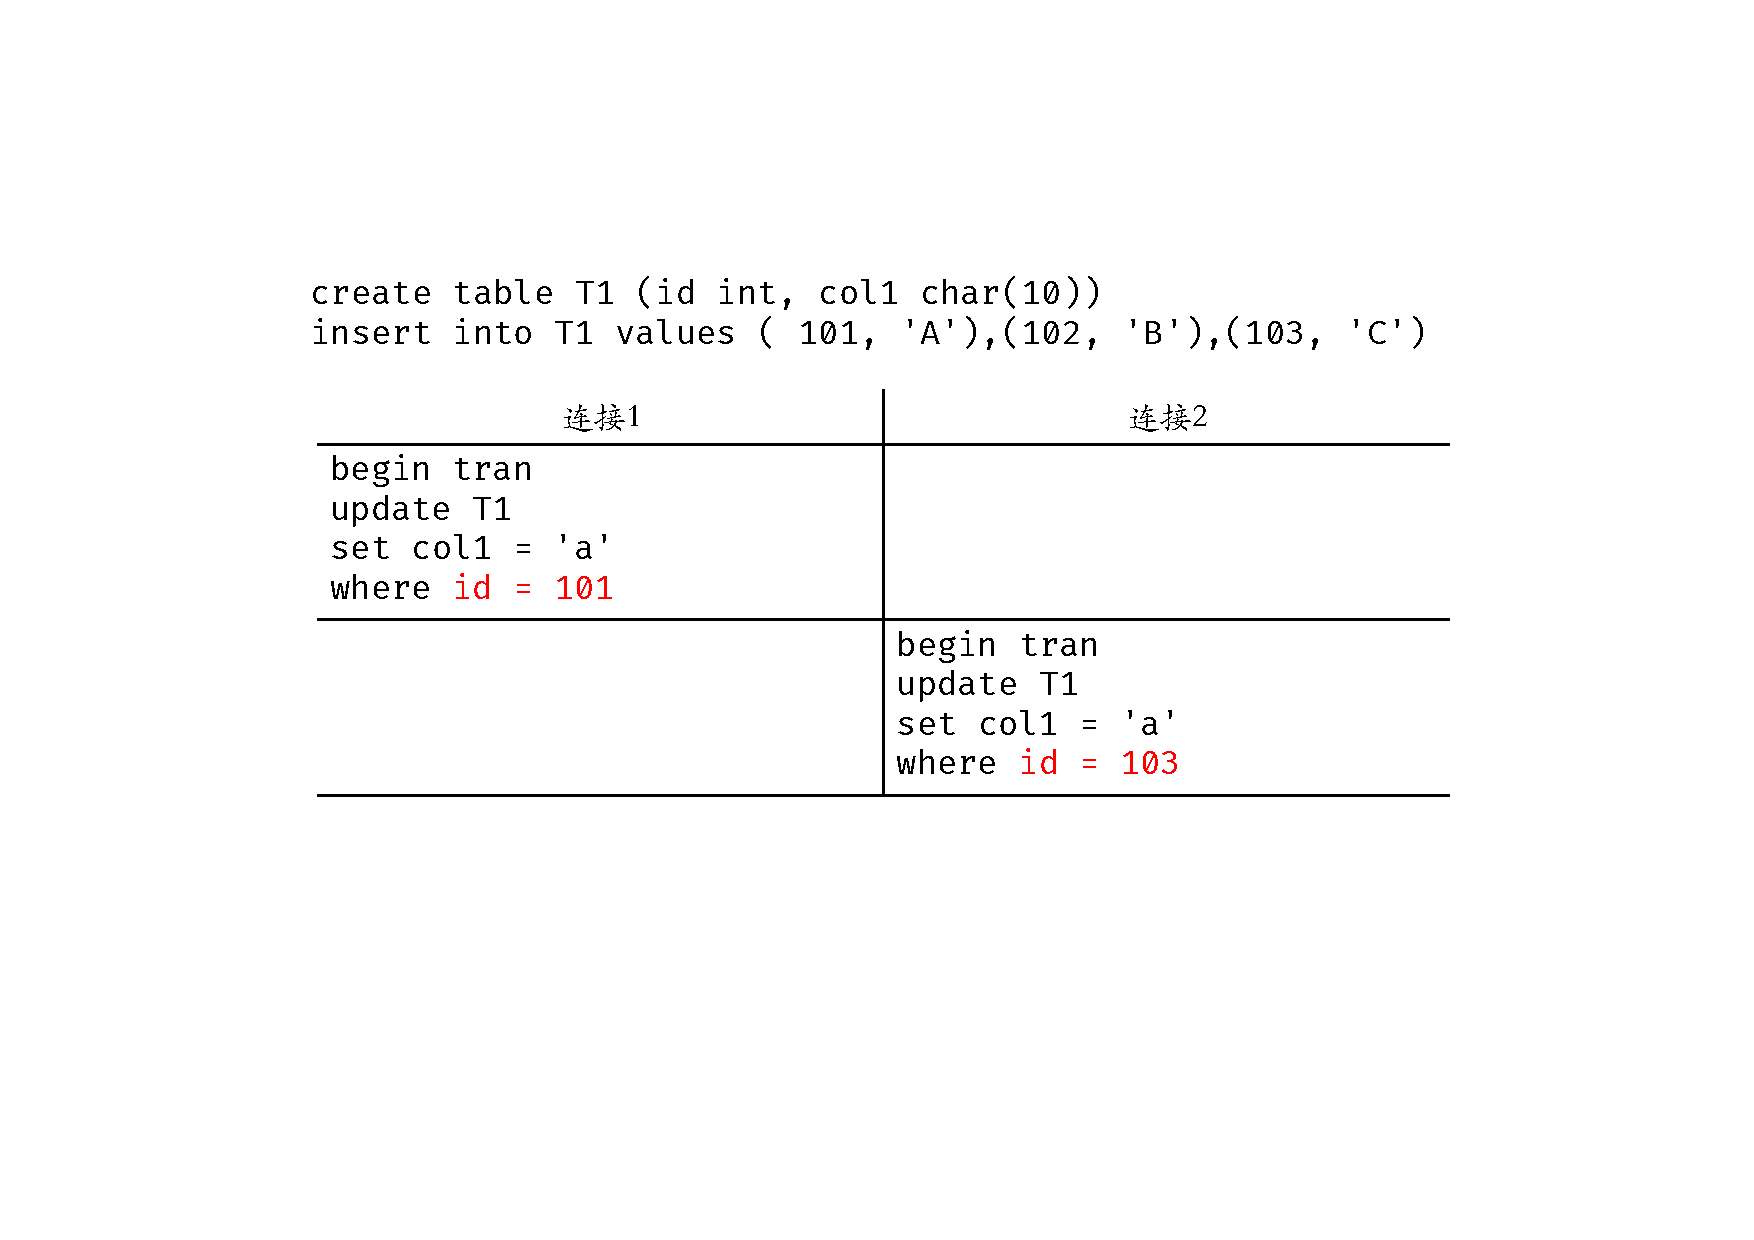
\includegraphics[width=.7\textwidth]{figure/阻塞.pdf}
    \caption{缺少索引引起的阻塞}
\end{figure}

\begin{enumerate}
    \item 连接1在表上没有找到索引, 因此进行全表的查询, 全部加U锁;
    \item 找到101, 升级为X锁, 释放其余的U锁;
    \item 连接2在表上没有找到索引, 因此进行全表的查询, 全部加U锁;
    \item 但是在试图对101加锁的时候和X锁冲突, 此时出现了\textcolor{red}{阻塞}.
\end{enumerate}

\subsubsection{死锁(Deadlock)}

两个事务都封锁了一些数据对象, 并相互等待对方
释放另一些数据对象以便对其封锁, 结果两个事务
都不能结束, 则发生死锁.

\begin{figure}[H]
    \centering
    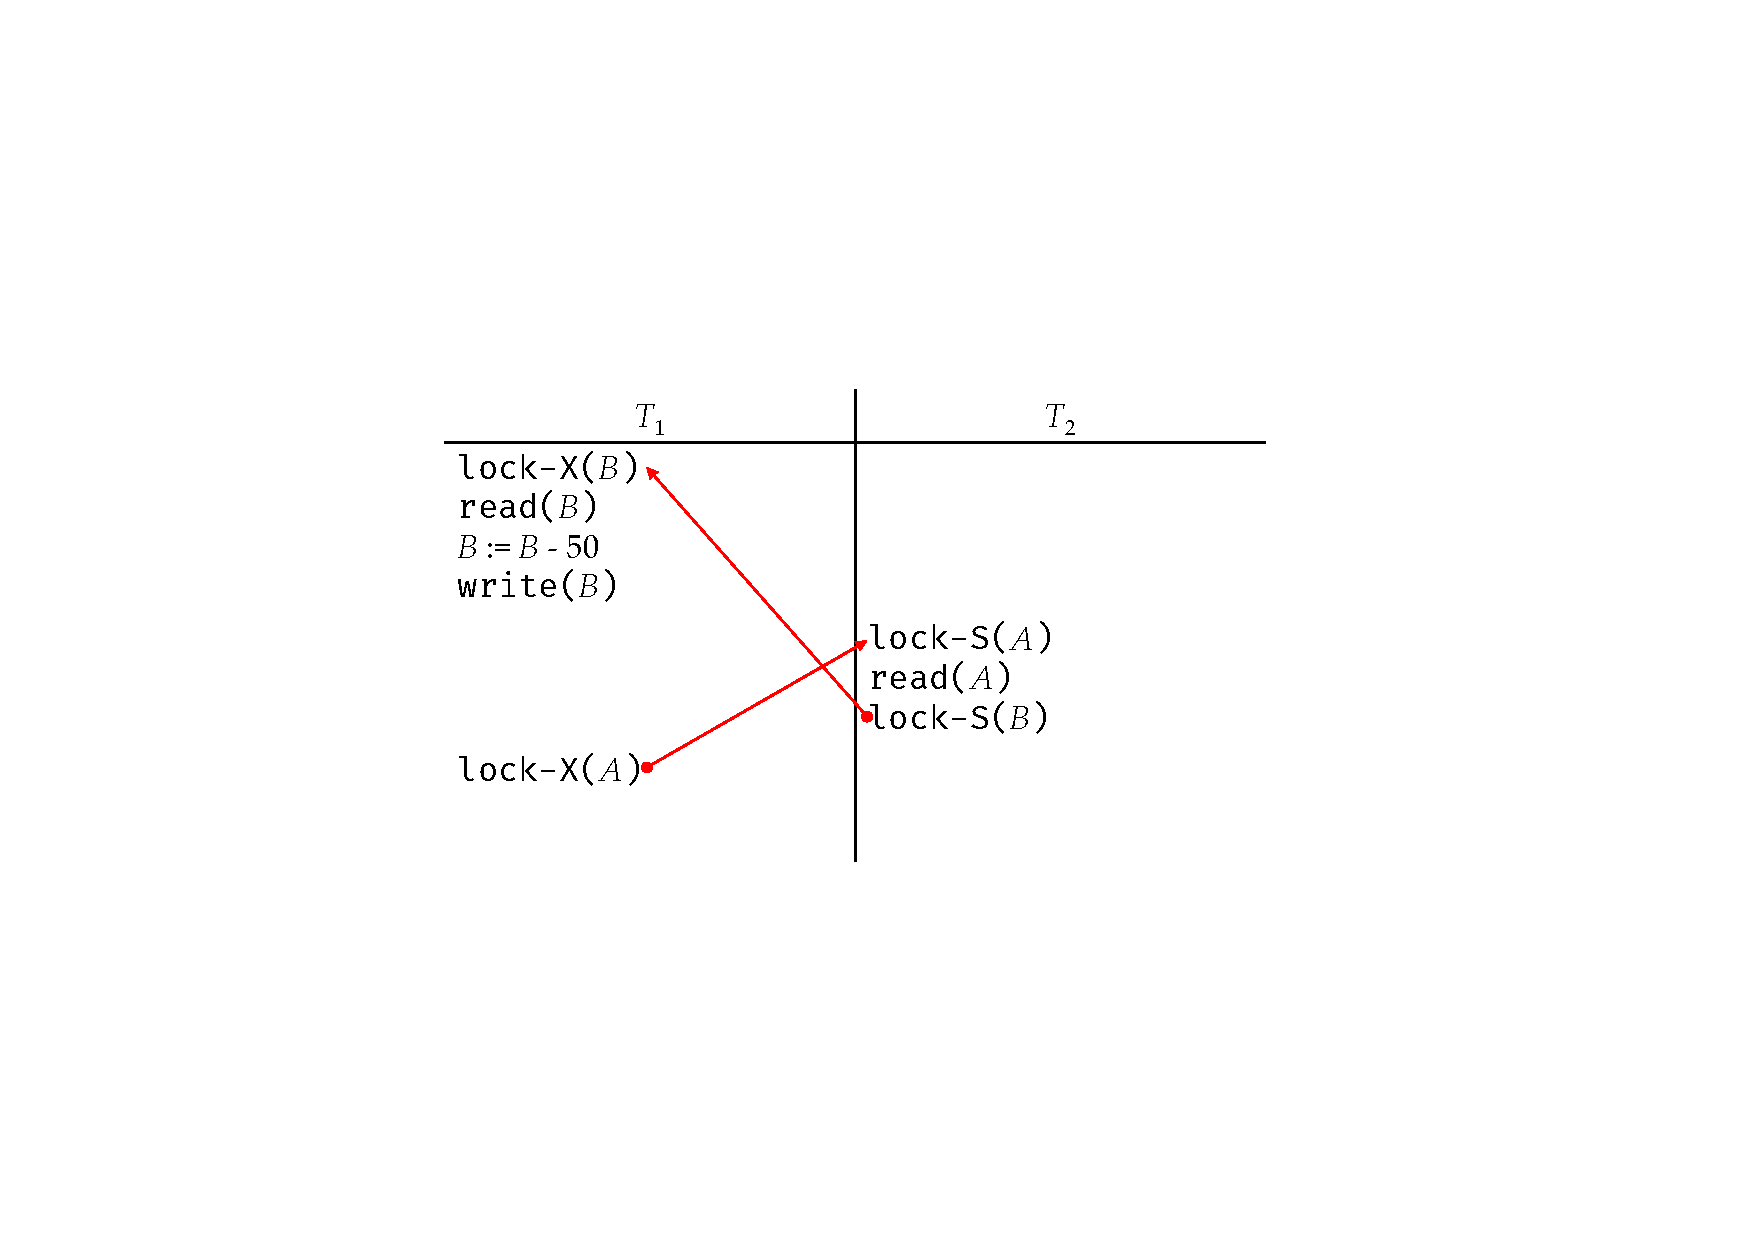
\includegraphics[width=.5\textwidth]{figure/死锁.pdf}
    \caption{死锁}
    \label{fig:deadlock}
\end{figure}

死锁发生的条件:
\begin{enumerate}
    \item \textcolor{red}{互斥条件}: 事务请求对资源的独占控制
    \item \textcolor{red}{占有等待条件}: 事务已持有一定资源, 又去申请并等待其它资源
    \item \textcolor{red}{非抢占条件}: 直到资源被持有它的事务释放之前, 不能将该资源强制从持有它的事务夺去
    \item \textcolor{red}{循环等待条件}: 存在事务相互等待的等待圈
\end{enumerate}

\begin{theorem}
  在条件1、2、3成立的前提下, 条件4是死锁存在的充分必要条件.
\end{theorem}

死锁检测: 构造事务之间的等待图. 事务$T_i$正在等待$T_j$则画一条有向边$T_i\to T_j$. 如果有环就说明有死锁.

如何避免死锁:
\begin{enumerate}
    \item 选择较低的隔离性级别
    \item 封锁粒度小一些
    \item 不同事物访问一组对象, 按照相同顺序访问
\end{enumerate}

\begin{remark}
  通常, 数据库系统会选择回滚较年轻的事务或者根据其他策略(如估计回滚成本)来决定哪个事务被回滚.

  也就是\ref{fig:deadlock}中会选择回滚$T_2$.
\end{remark}

\textbf{预防死锁: 破坏占有等待条件}

\begin{enumerate}
    \item 预先占据所需的全部资源: 要么一次全部封锁, 要么全不封锁.
    \begin{enumerate}
        \item 缺点: 难于预知需要封锁哪些数据并且数据使用率低
    \end{enumerate}
    \item 所有资源预先排序, 事务按规定顺序封锁数据.
\end{enumerate}

\textbf{预防死锁: 破坏非抢占条件}
\begin{enumerate}
    \item 使用抢占与事务回滚: 通过规定事务之间的优先级(老事务优先级高于新事务)来破坏死锁的非抢占条件.
\end{enumerate}

\begin{figure}[H]
    \centering
    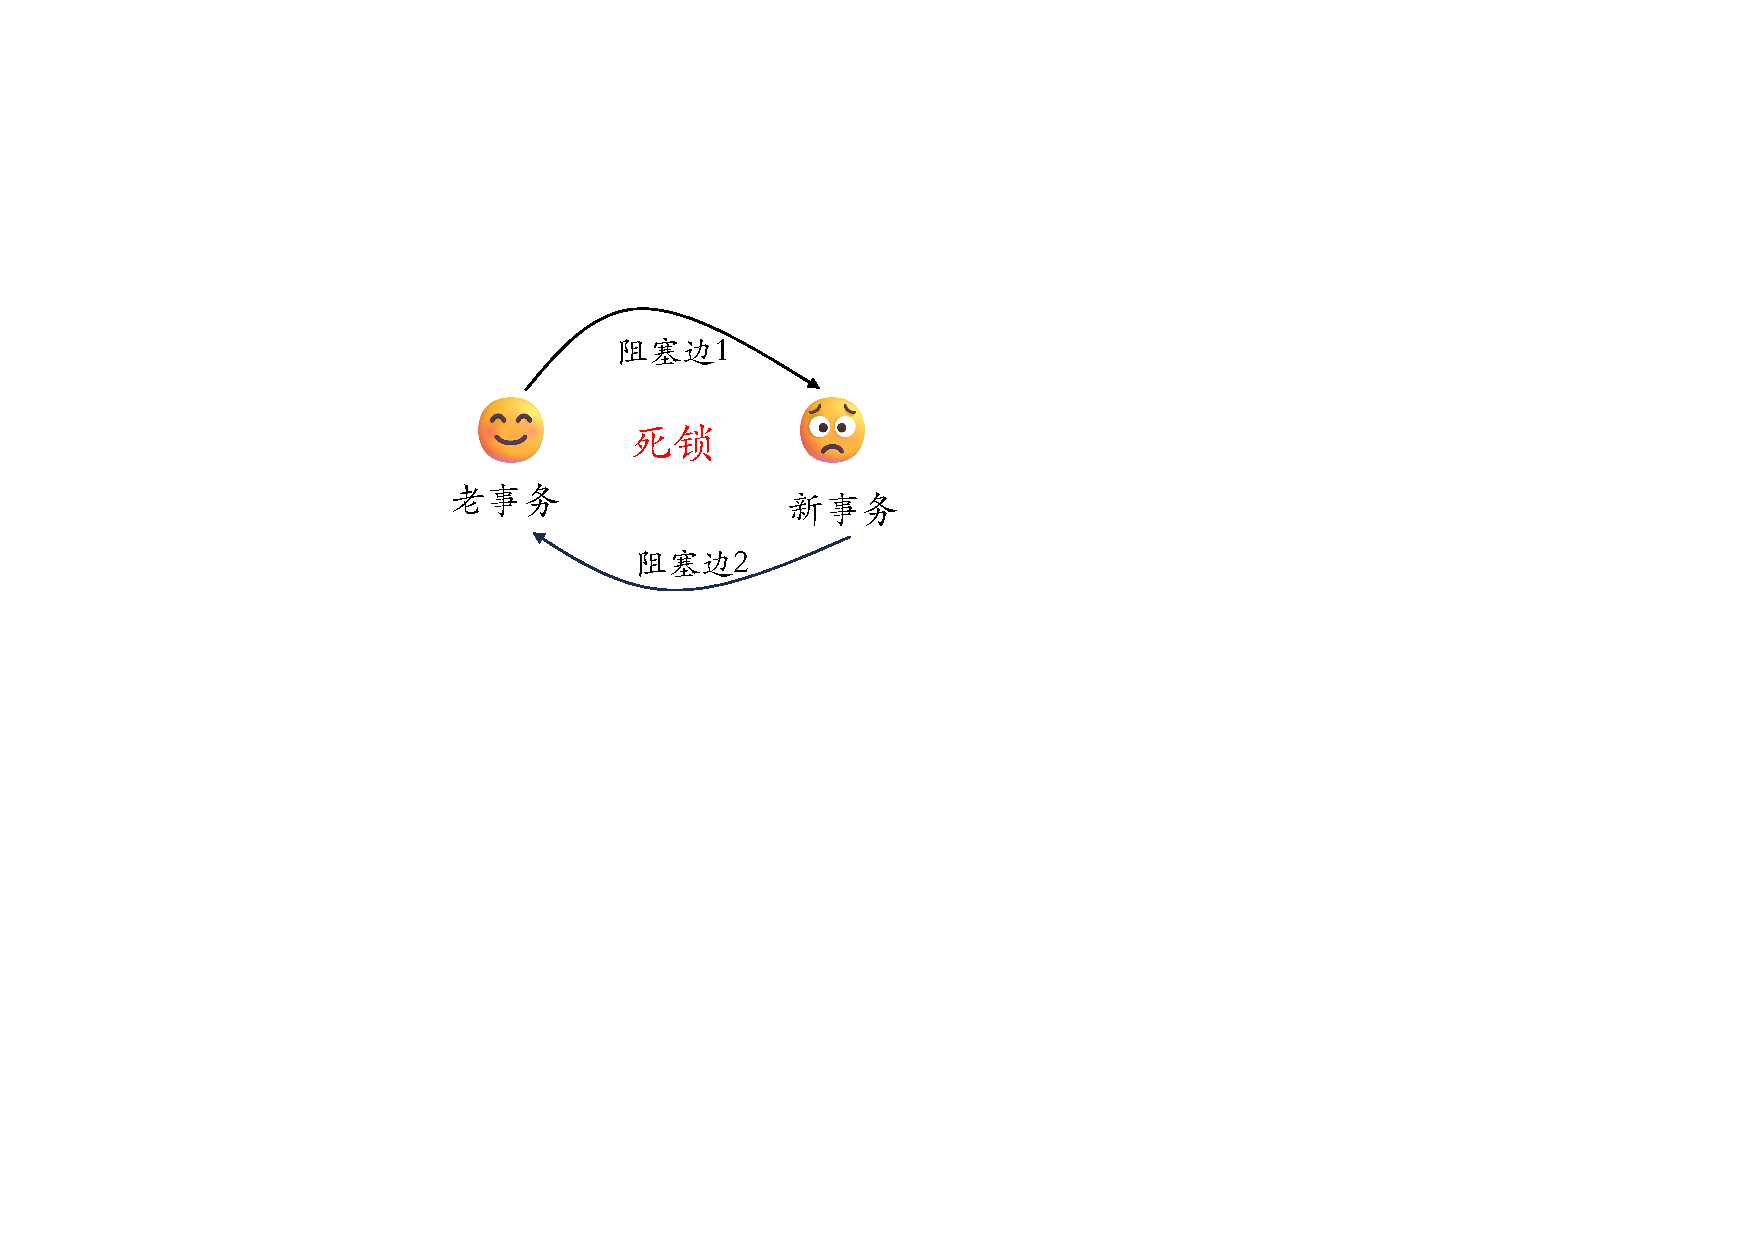
\includegraphics[width=.4\textwidth]{figure/死锁2.pdf}
    \caption{死锁出现的条件}
\end{figure}

\begin{enumerate}
    \item \textcolor{red}{wait-die}: 只允许老事务等待新事务(阻塞边1), 出现新事务等待老事务时(阻塞边2), 回滚新事务.
    \item \textcolor{red}{wound-wait}: 只允许新事务等待老事务(阻塞边2), 出现老事务等待新事务时(阻塞边1), 回滚\textcolor{red}{新事务}. \textit{老事务不等待, 直接杀死新事务.}
\end{enumerate}

\begin{example}
  对于调度$\text{start}(T_1), \text{start}(T_2), w_1(R_1), w_2(R_2), r_1(R_2), r_2(R_1)$, 分别使用wait-die或者wound-die来判断$T_2$在哪一步被回滚.
\end{example}

\textit{ 解答. }对于wait-die, 在$r_2(R_1)$的时候$T_2$开始等待, 被回滚. 对于wound-die, 在$r_1(R_2)$的时候$T_1$开始等待, 此时杀死$T_2$, $T_2$开始回滚.

死锁检测和恢复: 
\begin{enumerate}
    \item 超时法: 如果等待封锁的时间超过限时, 则撤消该事务.
    \item 等待图法: 在LOCK\_MONITOR中实现.
\end{enumerate}

\subsubsection{活锁 (Live lock)}

\begin{definition}[活锁(Live lock)]
  可能存在某个事务永远处于等待状态, 得不到执行, 称之为\textcolor{red}{活锁}(饿死).
\end{definition}

活锁的例子: 身处众多读锁中的写锁.

避免活锁的策略是遵从“先来先服务”的原则: 按请求封锁的顺序对各事务排队.

\subsection{其他锁相关概念}

\begin{definition}[锁管理器]
  \begin{itemize}
    \item 事务向锁管理器发送封锁请求和释放请求
    \item 锁管理器维护一个锁表记录锁的授予情况和处于等待状态的封锁请求
  \end{itemize}
\end{definition}

\begin{definition}[锁表]
  锁表一般作为内存中的hash表, 按被封锁对象的名字建立索引.
\end{definition}

...

"Unimportant. There's a million things I haven't done."

\section{基于时间戳的协议}

事务时间戳的分配:
\begin{itemize}
  \item 每个事务$T_i$进入系统被分配一个时间戳\textcolor{red}{$TS(T_i)$}.
  \item 如果$T_j$晚于$T_i$进入系统, 则\textcolor{red}{$TS(T_i)<TS(T_j)$}.
  \item 回滚的事务重新启动, 分配新的时间戳.
  \item 时间戳顺序决定了串行化顺序. \textcolor{red}{因此, 若$TS(T_i)<TS(T_j)$, 则系统必须保证所产生的调度等价于事务$T_i$出现在事务$T_j$之前的这样一个串行调度.}
  \item 回滚违反发出串行性操作的事务.
\end{itemize}

要实现这样一种机制, 我们将每个数据项$Q$与两个时间戳值相关联:
\begin{enumerate}
    \item $WT(Q)$: 所有执行$\text{write}(Q)$的事务中最大的时间戳;
    \item $RT(Q)$: 所有执行$\text{read}(Q)$的事务中最大的时间戳.
\end{enumerate}

同时为了避免可能的脏读, 我们为数据项$Q$设置提交位$C(Q)$: 表示拥有$Q$上写时间戳的事务是否提交.

\begin{definition}[时间戳排序协议(timestamp-ordering protocol)]
  保证任何有冲突的 read 和 write 操作按时间戳的次序执行, 该协议运作方式如下:
  \begin{itemize}
    \item 假设事务$T_i$发出$\text{read}(Q)$.
    \begin{itemize}
      \item 如果$TS(T_i)<WT(Q)$: $T_i$需读入的值已经被覆盖, $\text{read}(Q)$操作被拒绝, 回滚$T_i$;
      \item 如果$TS(T_i)\geq WT(Q)$: 
      \begin{itemize}
        \item 若$C(Q)$为真, 则执行$\text{read}(Q)$操作, $RT(Q)=\max(RT(Q), TS(T_i))$;
        \item 若$C(Q)$为假, 则推迟到$C(Q)$为真或者写$Q$的事务中止.
      \end{itemize}
    \end{itemize}
    \item 假设事务$T_i$发出$\text{write}(Q)$.
    \begin{itemize}
      \item 如果$TS(T_i)<RT(Q)$: $T_i$产生的值是先前所需要的值, $\text{write}(Q)$操作被拒绝, 回滚$T_i$;
      \item 如果$TS(T_i)<WT(Q)$: $T_i$产生的值已经被其后的写事务覆盖, 跳过$T_i$的$\text{write}(Q)$; (\textcolor{red}{Thomas写规则: 写操作在更晚的写操作已经发生时可以跳过.})
      \item 如果$TS(T_i)>RT(Q) \land TS(T_i) > WT(Q)$, 则执行$T_i$的$\text{write}(Q)$, $WT(Q)=TS(T_i)$.
    \end{itemize}
  \end{itemize}
\end{definition}

如何实现时间戳?
\begin{enumerate}
    \item 计数器
    \item 向量时钟
    \item 物理时钟
    \item 逻辑时钟
\end{enumerate}


\begin{figure}[H]
    \centering
    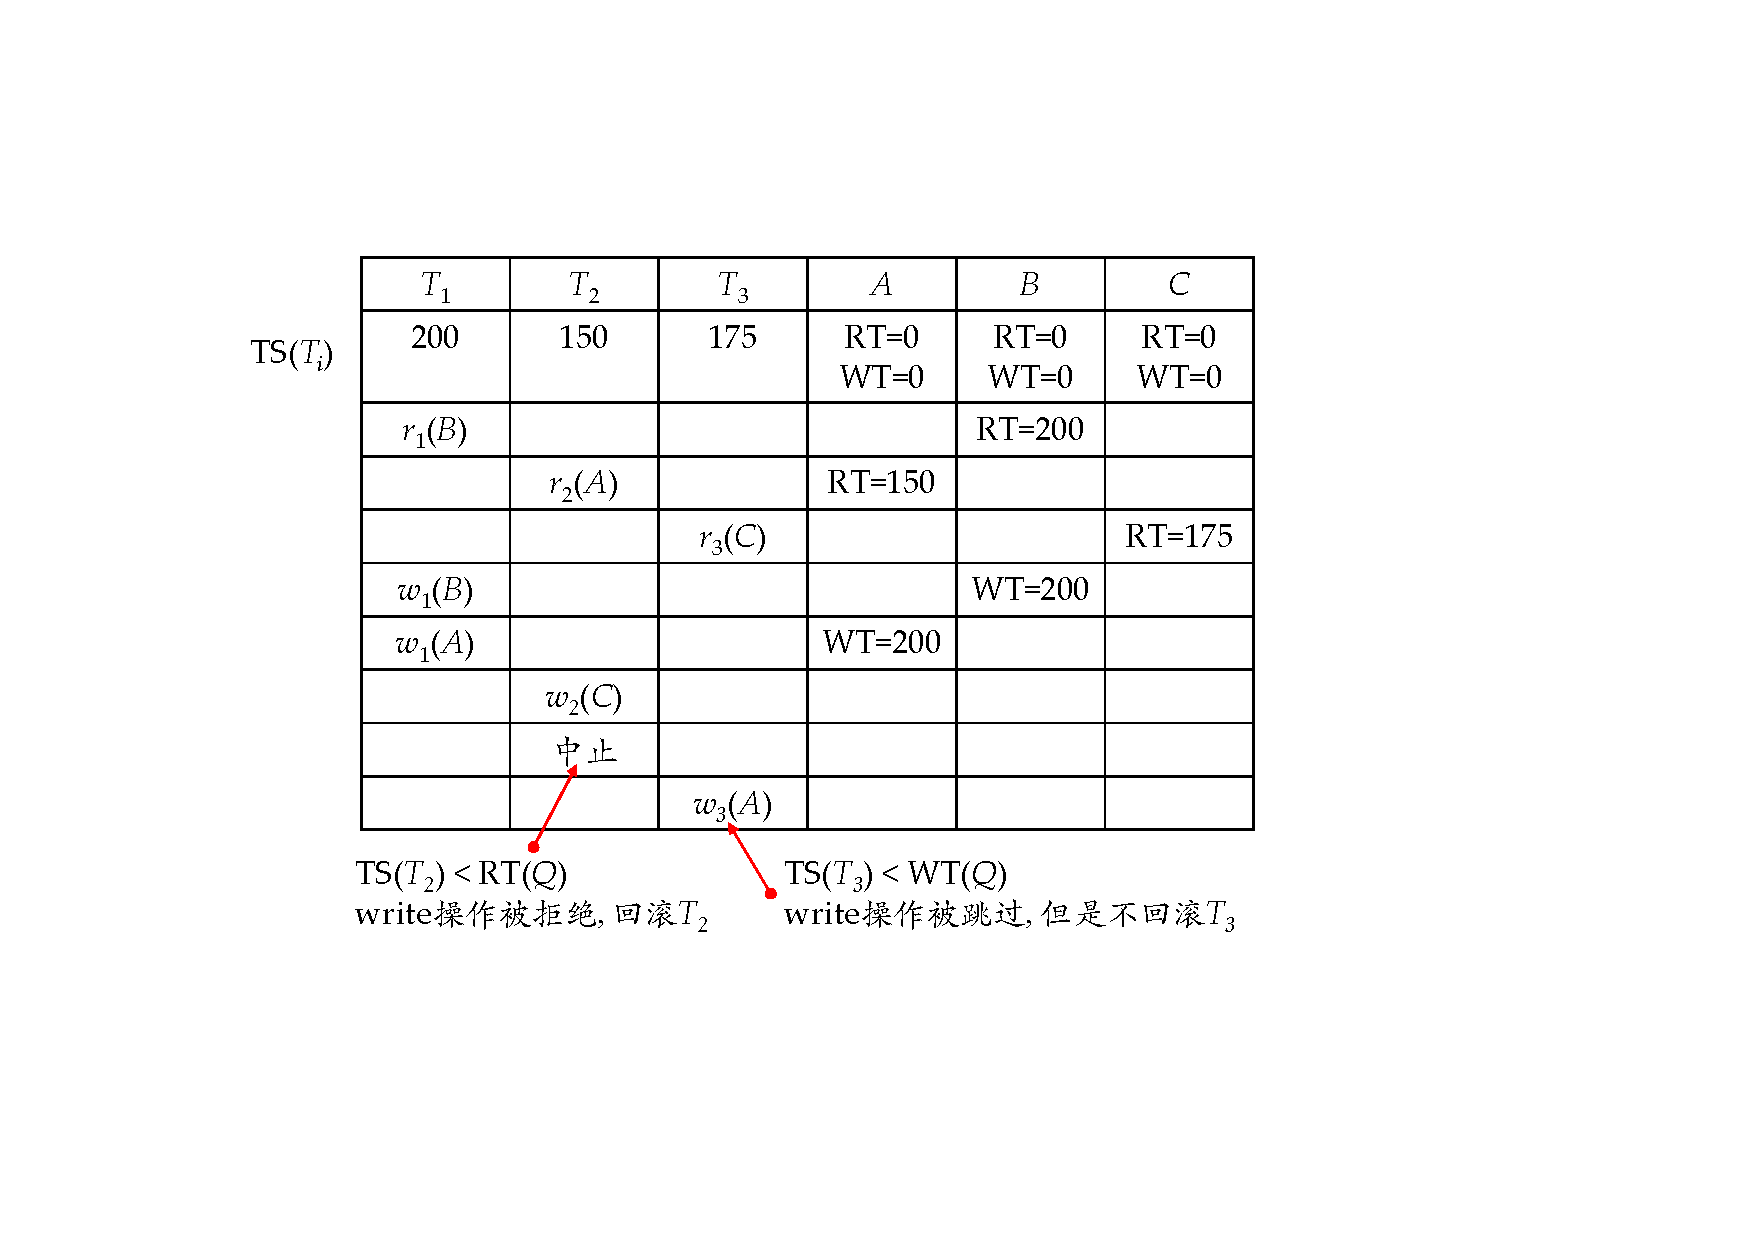
\includegraphics[width=.7\textwidth]{figure/时间戳.pdf}
    \caption{基于时间戳协议的练习}
\end{figure}

\section{基于有效性检查的协议}

在大部分事务是只读事务的情况下, 事务之间发生冲突的概率较低. 所以即使没有并发控制机制, 也可以达到一致性. $\to$ 采用减小并发开销的可替代方案可能是更好的.

减小开销所面临的困难是我们事先并不知道哪些事务将陷入冲突中, 为获得这种知识, 我们需要一种监控 (monitoring) 系统的机制.

\begin{definition}[有效性检查协议 (validation protocol)]
有效性检查协议 (validation protocol) 要求每个事务$T_i$在其生命周期中按两个或三个不
同的阶段执行, 这取决于该事务是一个只读事务还是一个更新事务.
\begin{itemize}
  \item 读阶段. 在这一阶段中, 系统执行$T_i$. 它读取各数据项的值并将它们保存在$T_i$的局部变量中, $T_i$的所有write操作都是对\textcolor{red}{局部的临时变量}进行的, 并不对数据库进行真正的更新.
  \item 有效性检查阶段. 对事务$T_i$进行有效性检查的测试(见下文). 这将决定是否允许$T_i$继续执行到写阶段而不违反可串行性. 如果事务的有效性检查的测试失败, 则系统终止这个事务.
  \item 写阶段. 若事务$T_i$通过了有效性检查的测试, 则保存$T_i$所执行的任何 write 操作结果的临时局部变量被拷入数据库. 对于只读事务忽略这个阶段.
\end{itemize}
\end{definition}

\textcolor{red}{并发执行事务的 三个阶段是可以交叉执行的!}

\textbf{有效性检查的测试}:
\begin{itemize}
  \item 我们将三个不同的时间戳与每个事务$T_i$相关联:
  \begin{enumerate}
      \item $StartTS(T_i)$: 事务$T_i$开始其执行的时间;
      \item $ValidationTS(T_i)$: 事务$T_i$完成其读阶段并开始其有效性检查阶段的时间;
      \item $FinishTS(T_i)$: 事务$T_i$完成其写阶段的时间.
  \end{enumerate}
  \item 我们令$TS(T_i)=ValidationTS(T_i)$, 并且若$TS(T_j)<TS(T_k)$, 则产生的任何调度必须等价于其中事务$T_j$出现在事务$T_k$之前的一个串行调度.
  \item 有效性协议的检查条件, 我们假设$T_1$已确认, $T_2$待确认.
  \begin{enumerate}
      \item $StartTS(T_2)<FinishTS(T_1)<ValidationTS(T_2)$: 检查$RS(T_2)\cap WS(T_2) = \varnothing$. 
      \item $ValidationTS(T_2)<FinishTS(T_1)$: 检查$WS(T_2)\cap WS(T_1) = \varnothing \land RS(T_2) \cap WS(T_1) = \varnothing$.
  \end{enumerate}
\end{itemize}

\begin{figure}[H]
    \centering
    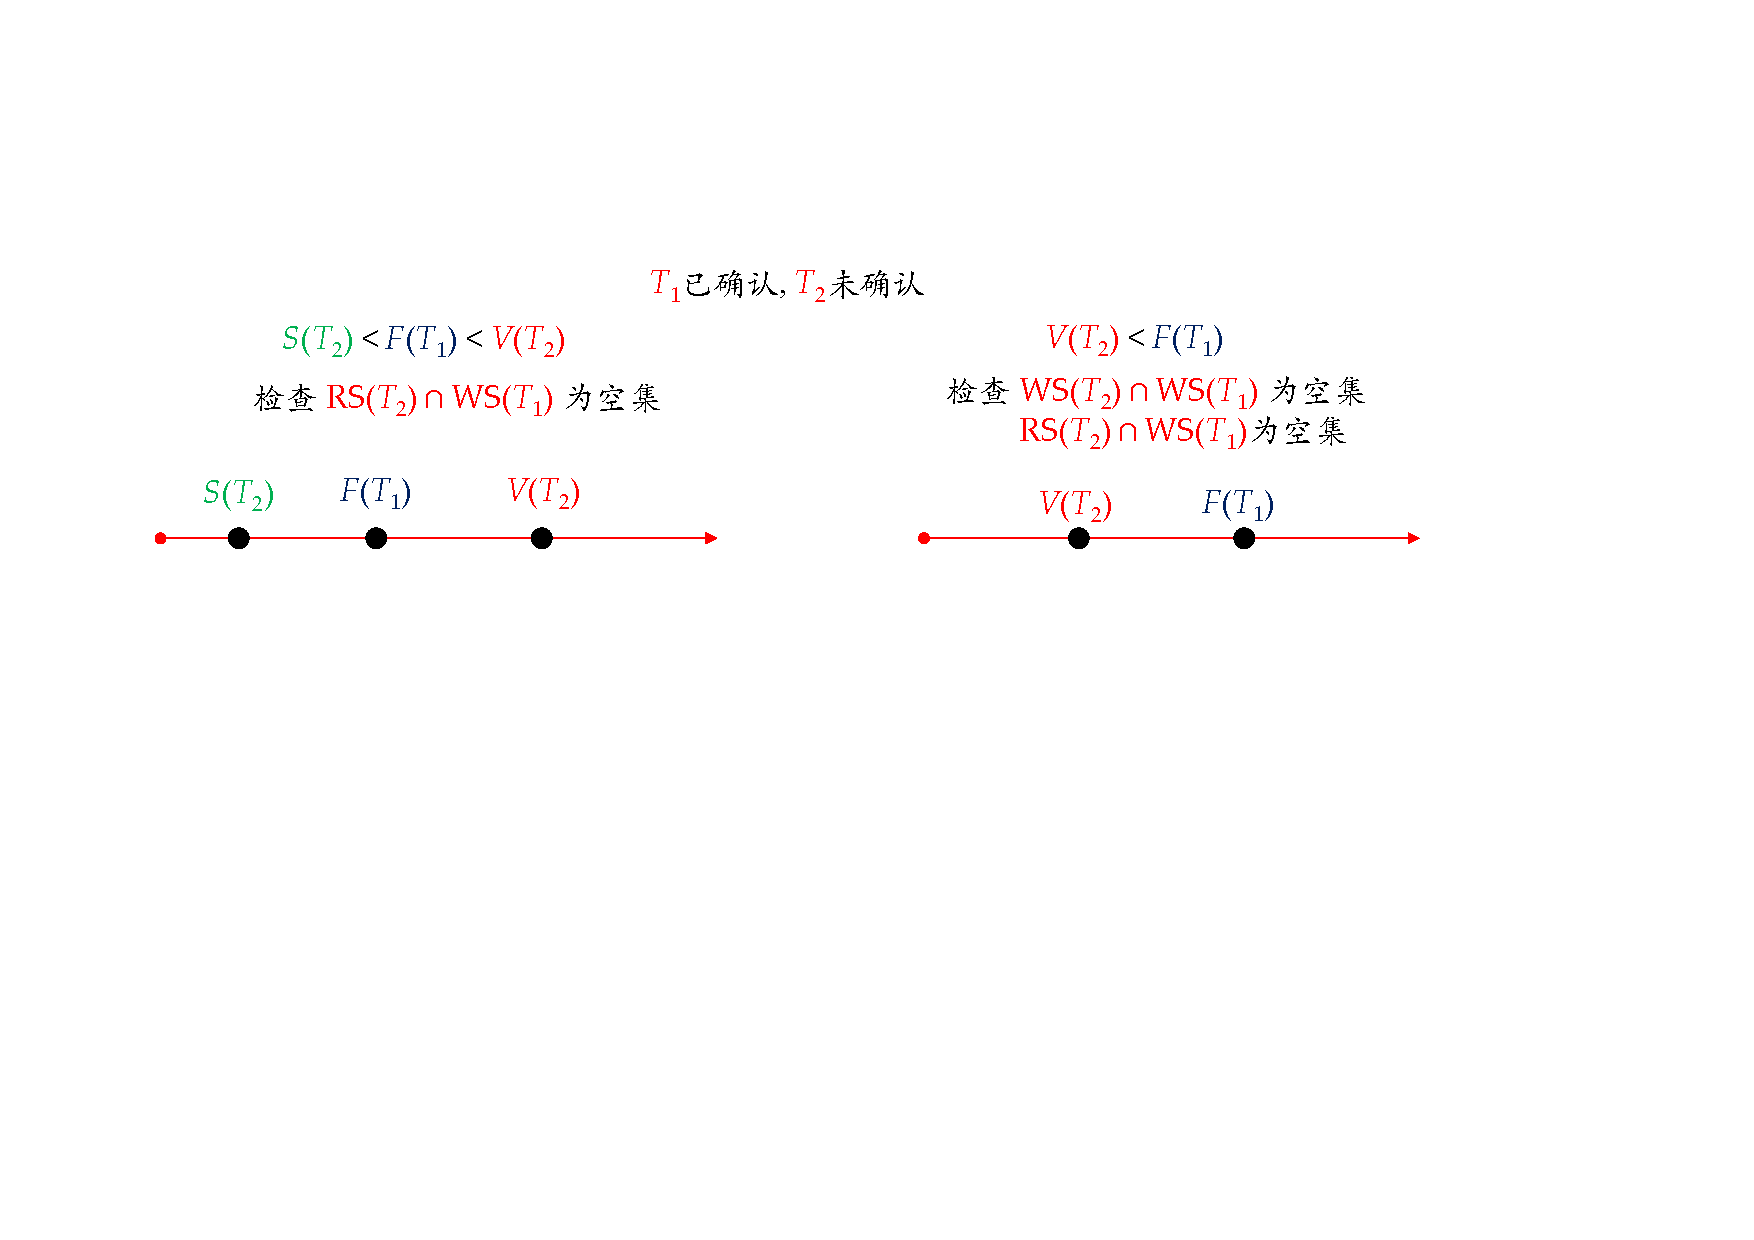
\includegraphics[width=.8\textwidth]{figure/有效性.pdf}
    \caption{有效性协议的检查条件}
\end{figure}

\begin{figure}[H]
    \centering
    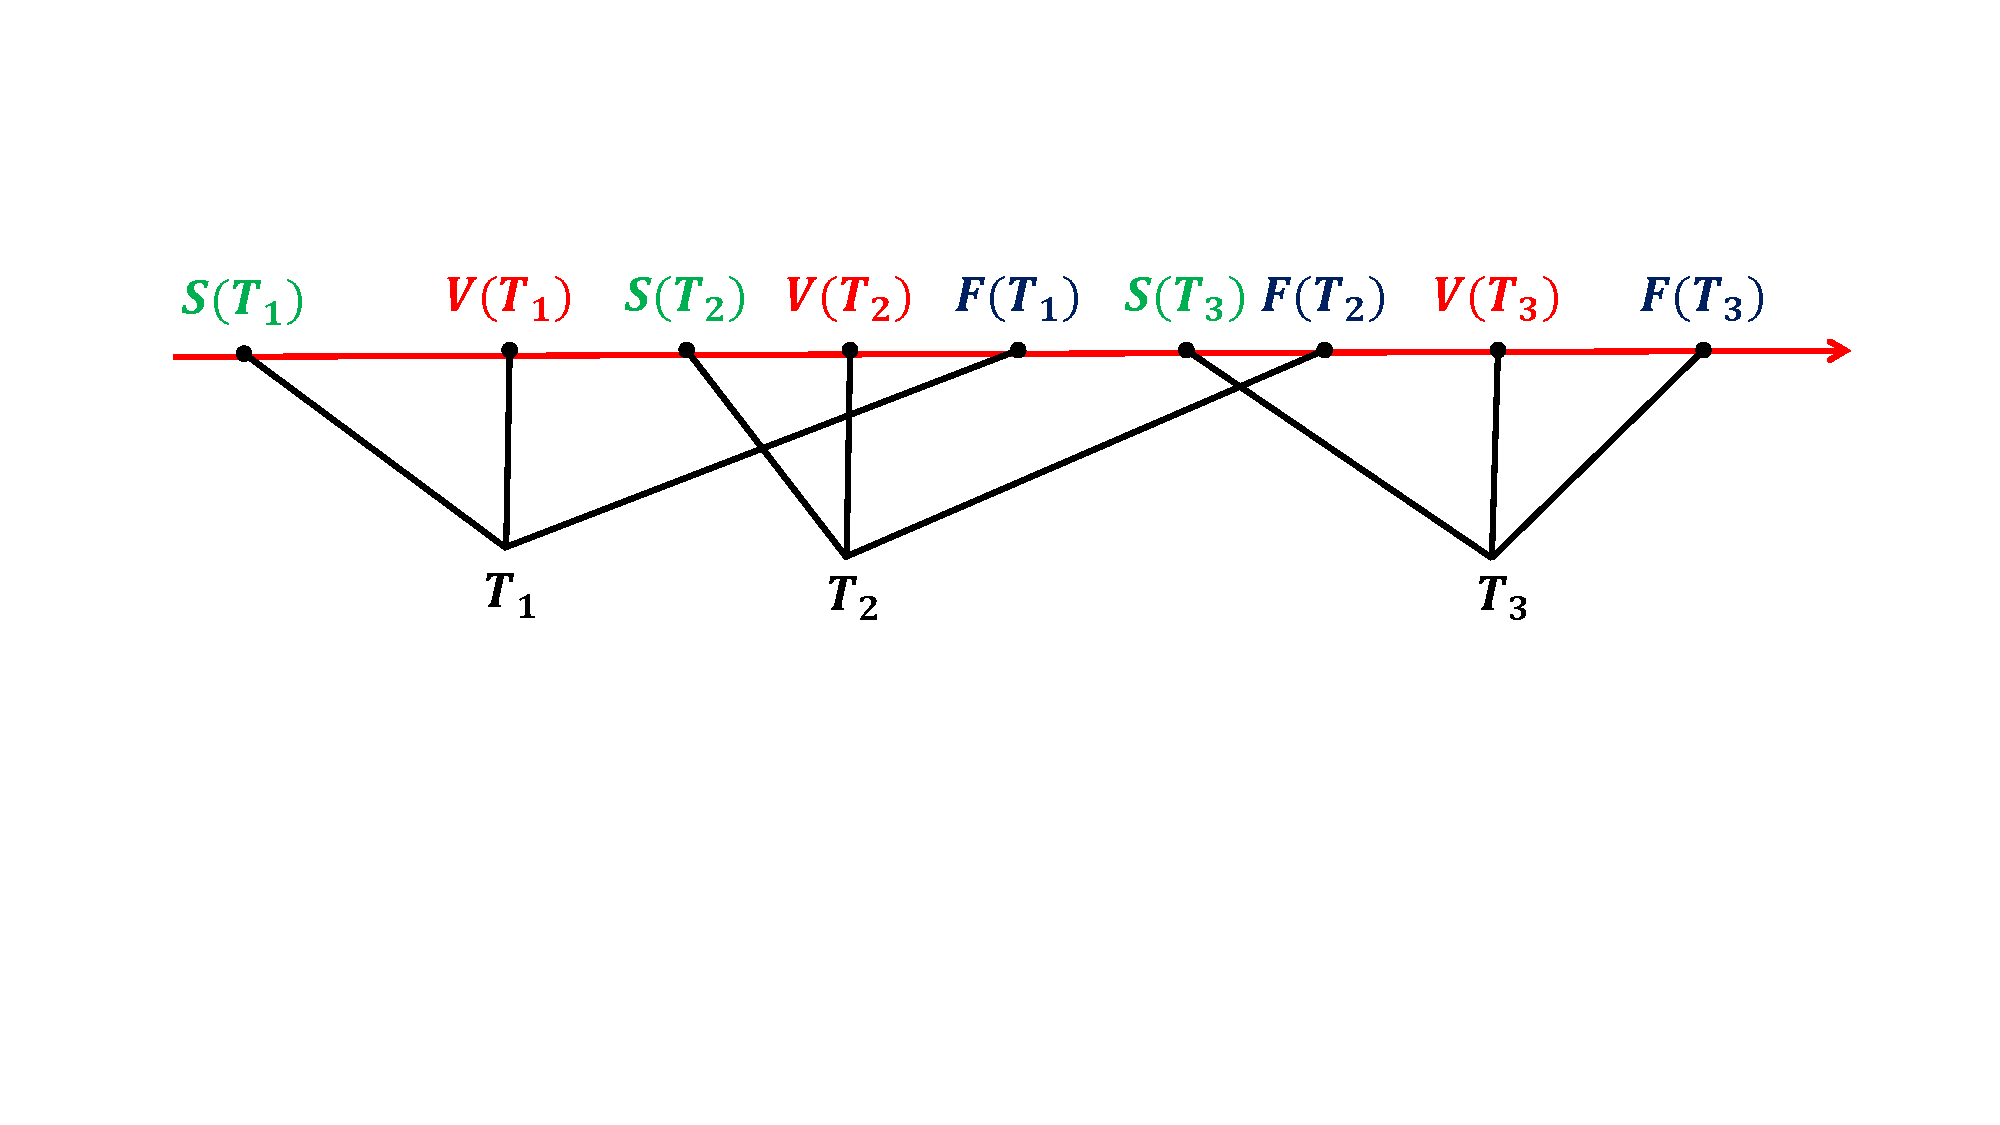
\includegraphics[width=.7\textwidth]{figure/有效性-例子.pdf}
    \caption{有效性检查协议的例子}
\end{figure}

确认$T_2$:
\begin{itemize}
  \item $S(T_2)<F(T_1)$: 检查$RS(T_2)\cap WS(T_1) = \varnothing$是否成立;
  \item $V(T_2)<F(T_1)$: 检查$WS(T_2) \cap WS(T_1) = \varnothing$是否成立.
\end{itemize}

确认$T_3$:
\begin{itemize}
  \item $S(T_3)>F(T_1)$: 不需要判定$T_3$和$T_1$的相交性;
  \item $S(T_3)<F(T_2)$: 检查$RS(T_3)\cap WS(T_2) = \varnothing$是否成立.
\end{itemize}

\section{MVCC(Multi-Version Concurrency Control)}

MVCC: Multi-Version Concurrency Control, 多版本并发控制.

\textbf{数据行结构}:
InnoDB每行数据增加三个隐藏列用于实现MVCC:
\begin{itemize}
  \item db\_trx\_id: 插入或更新行的最后一个事务的全局标识符(每个事务创建都会分配id, 全局递增)
  \item db\_roll\_ptr: 指向当前记录的前一个undo log版本
  \item db\_row\_id: 行标识(隐藏单调自增id)
\end{itemize}

\begin{figure}[H]
    \centering
    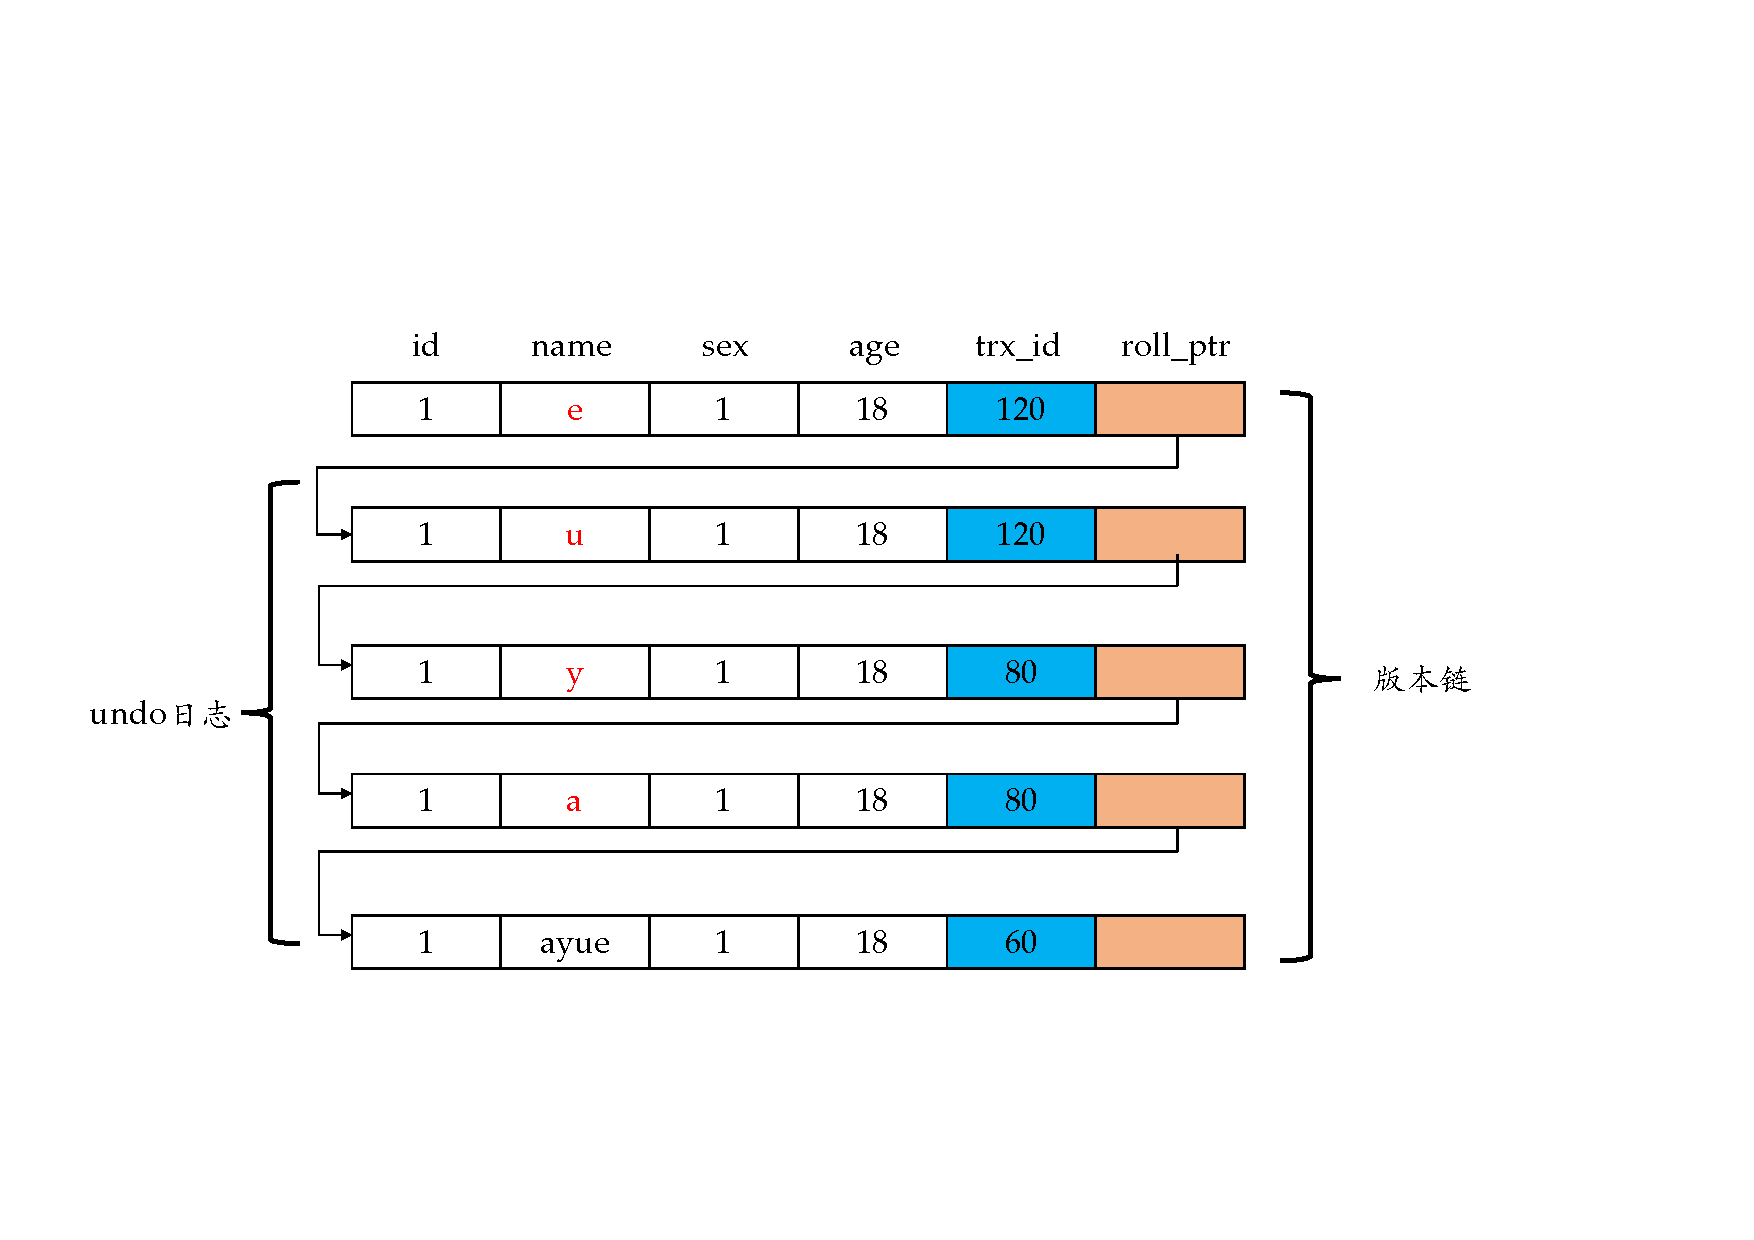
\includegraphics[width=.8\textwidth]{figure/MVCC.pdf}
    \caption{MySQL MVCC实现: 数据行}
\end{figure}

\textbf{读视图}: 事务在进行快照读的时候会创建一个读视图read\_view.
\begin{itemize}
  \item current\_trx\_id: 当前事务的id;
  \item alive\_trx\_list: 读视图生成时刻系统中正在活跃的事务id;
  \item min\_trx\_id: 上面的alive\_trx\_list中的最小事务id;
  \item max\_trx\_id: 读视图生成时刻目前已创建过的事务id最大值 + 1.
\end{itemize}


\textbf{可见性算法}: 

当一个事务读取某条记录$\text{record}_i$时会追溯其undo log版本链, 找到第一个可以访问的版本, 而该记录的某一个版本\textcolor{red}{db\_trx\_id($\text{record}_i$)}是否能被这个事务读取到遵循如下\textcolor{red}{可见性算法规则}:
\begin{figure}[H]
    \centering
    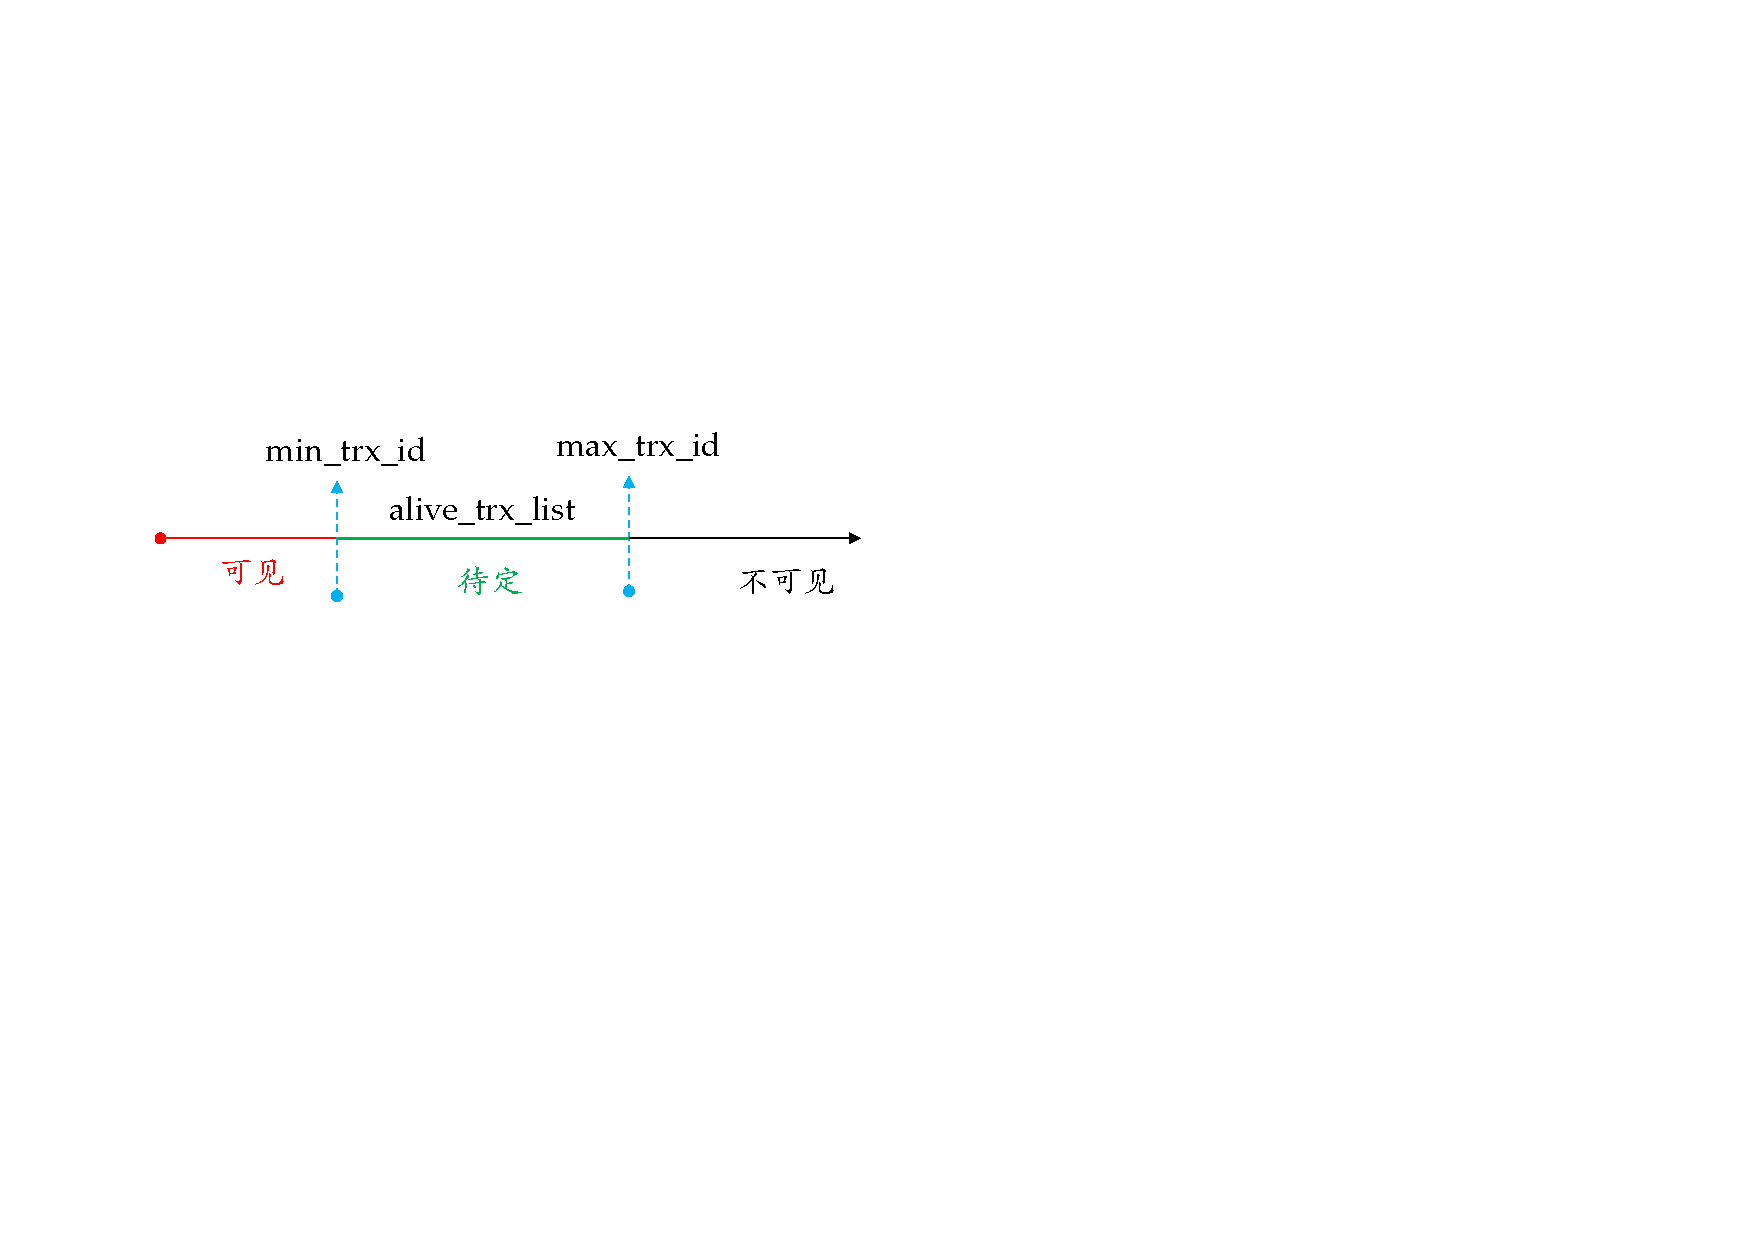
\includegraphics[width=.5\textwidth]{figure/可见性算法规则.pdf}
    \caption{可见性算法规则}
\end{figure}
\begin{itemize}
  \item 当$\text{db\_trx\_id}(\text{record}_i)<\text{min\_trx\_id}$时, 那么$\text{record}_i$对于当前事务可见(db\_trx\_id在当前事务之前提交);
  \item 当$\text{db\_trx\_id}(\text{record}_i)=\text{current\_trx\_id}$, 那么$\text{record}_i$对于当前事务可见(db\_trx\_id是被当前事务自身生成或修改的);
  \item 当$\text{db\_trx\_id}(\text{record}_i)>\text{max\_trx\_id}$时, 那么$\text{record}_i$对于当前事务不可见(db\_trx\_id在当前事务之后提交);
  \item 当$\text{min\_trx\_id}\leq \text{db\_trx\_id}(\text{record}_i)<\text{max\_trx\_id}$时, 而且$\text{db\_trx\_id}(\text{record}_i) \in \text{alive\_trx\_list}$, 那么$\text{record}_i$对于当前事务不可见(db\_trx\_id属于则说明这条记录还未提交, 对于当前操作的事务是不可见的);
  \item 当$\text{min\_trx\_id}\leq \text{db\_trx\_id}(\text{record}_i)<\text{max\_trx\_id}$时, 而且$\text{db\_trx\_id}(\text{record}_i) \not\in \text{alive\_trx\_list}$, 那么$\text{record}_i$\textcolor{red}{对于当前事务可见}(db\_trx\_id不属于则说明这条记录已经提交, 对于当前操作的事务是可见的).
\end{itemize}

\begin{figure}[H]
    \centering
    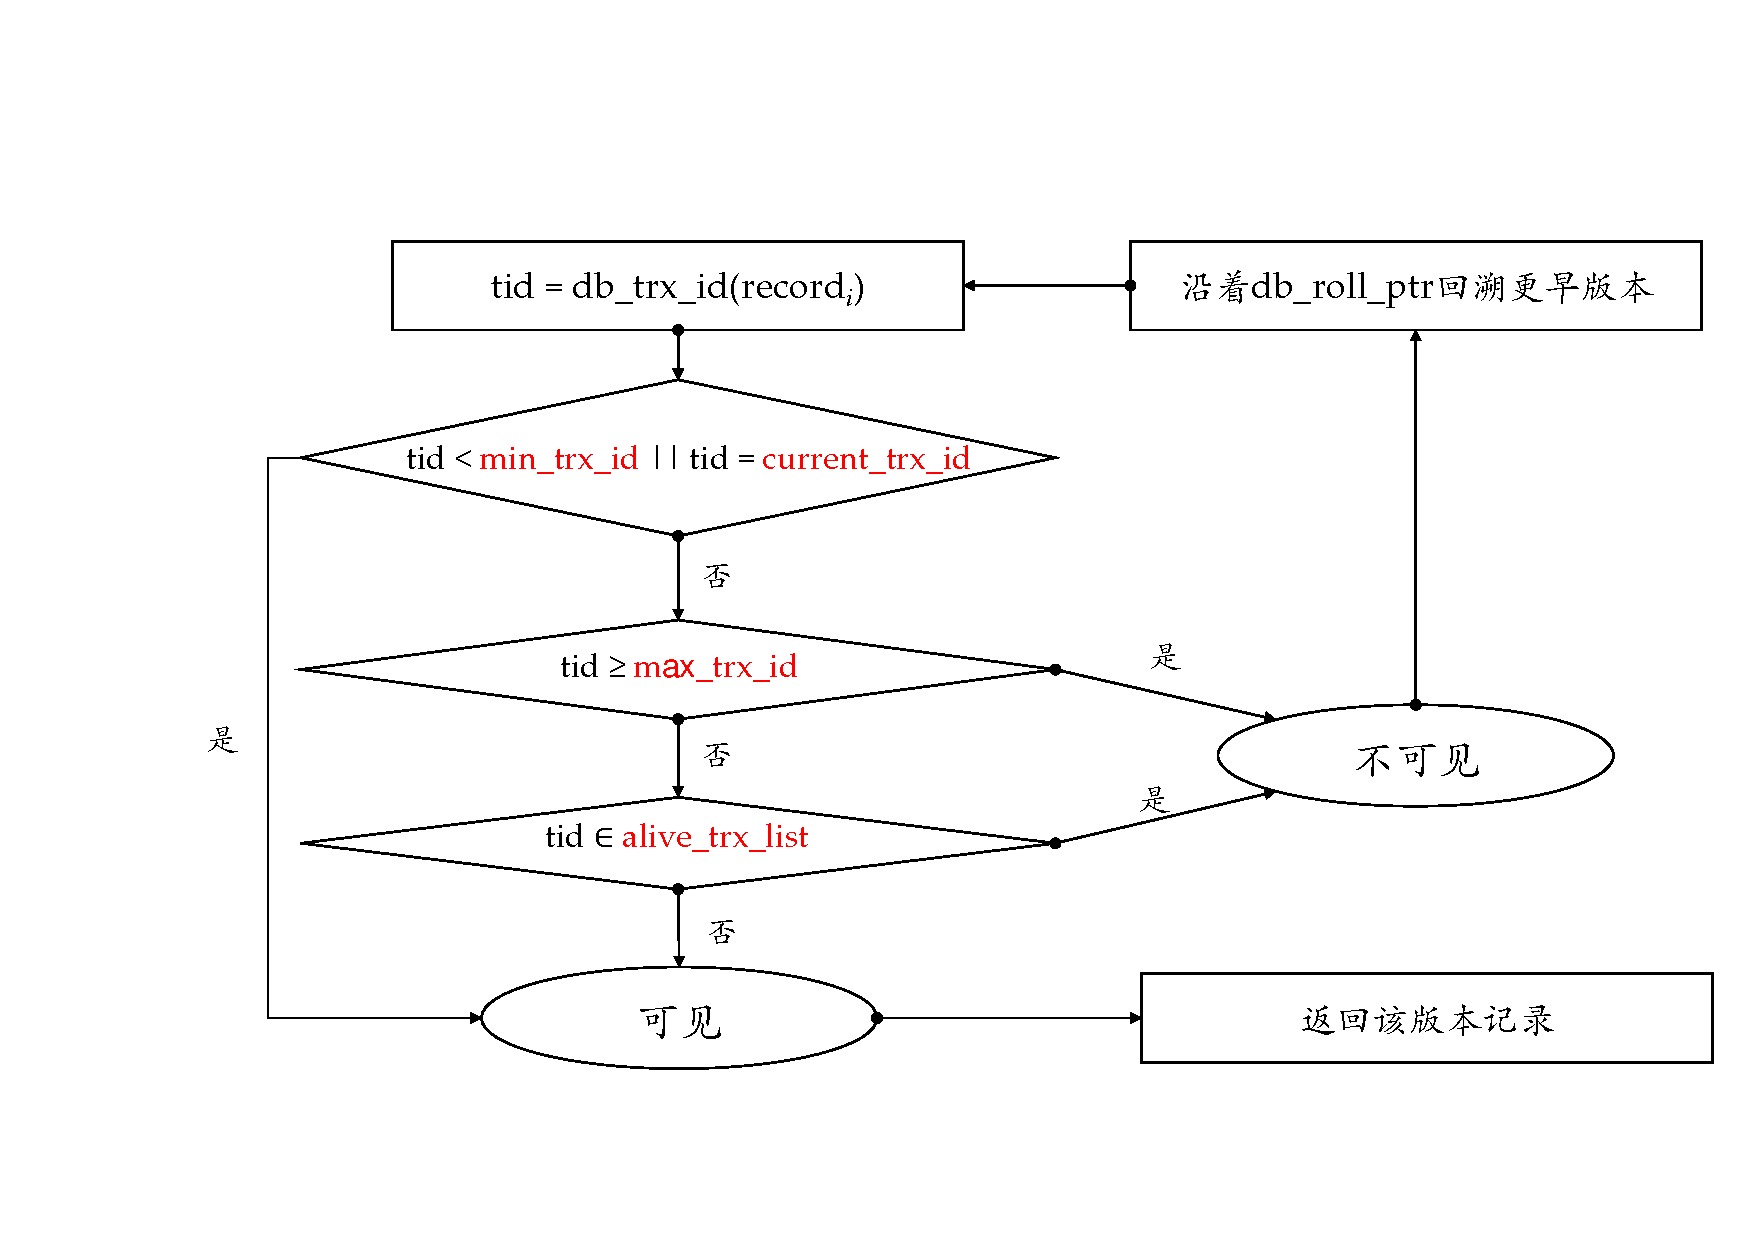
\includegraphics[width=.8\textwidth]{figure/可见性流程图.pdf}
    \caption{可见性算法规则流程图}
\end{figure}

\subsection{MySQL MVCC在不同隔离性级别下的读视图}

假设对于下面的两个事务$T_A$和$T_B$, 有下面的调度:
\begin{figure}[H]
    \centering
    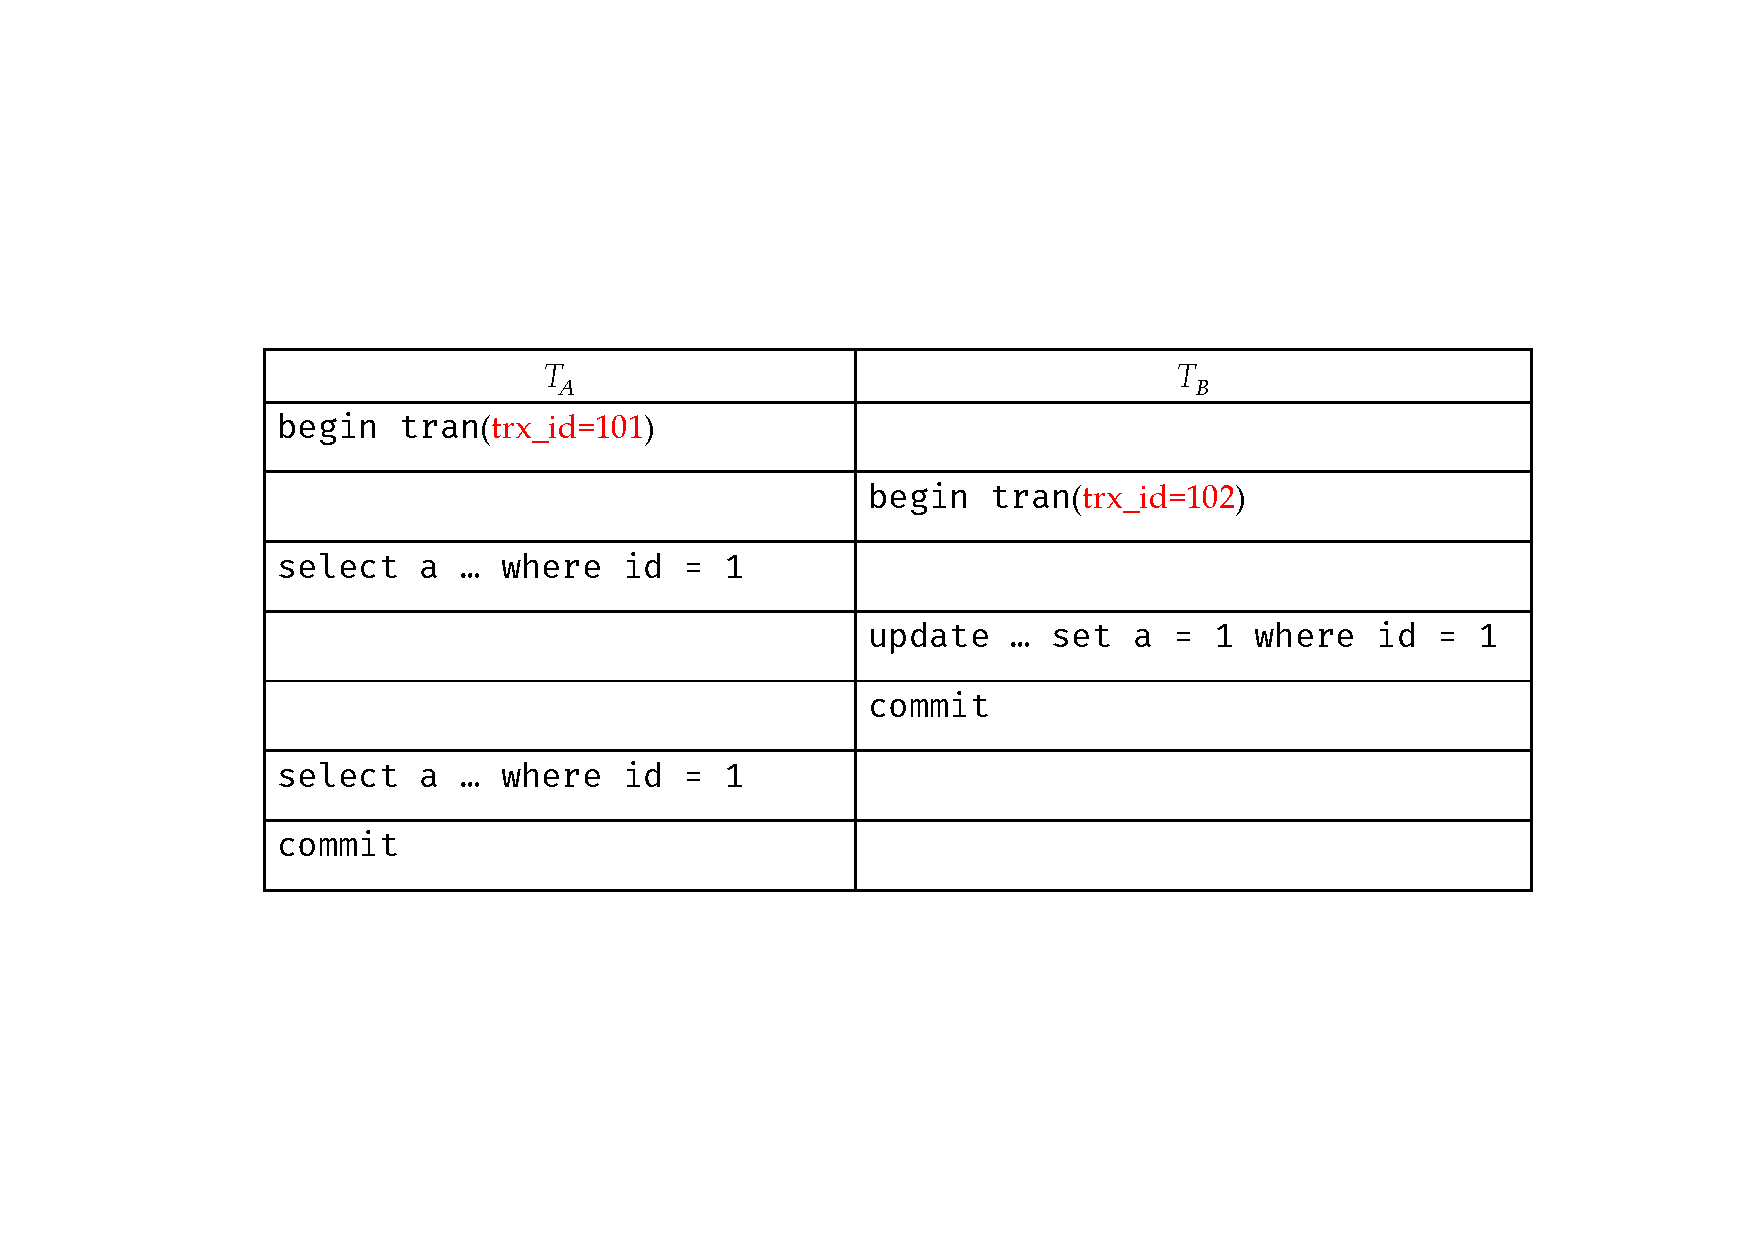
\includegraphics[width=.8\textwidth]{figure/MVCC-shiwu.pdf}
    \caption{MySQL MVCC的一个例子}
\end{figure}

\begin{figure}[H]
    \centering
    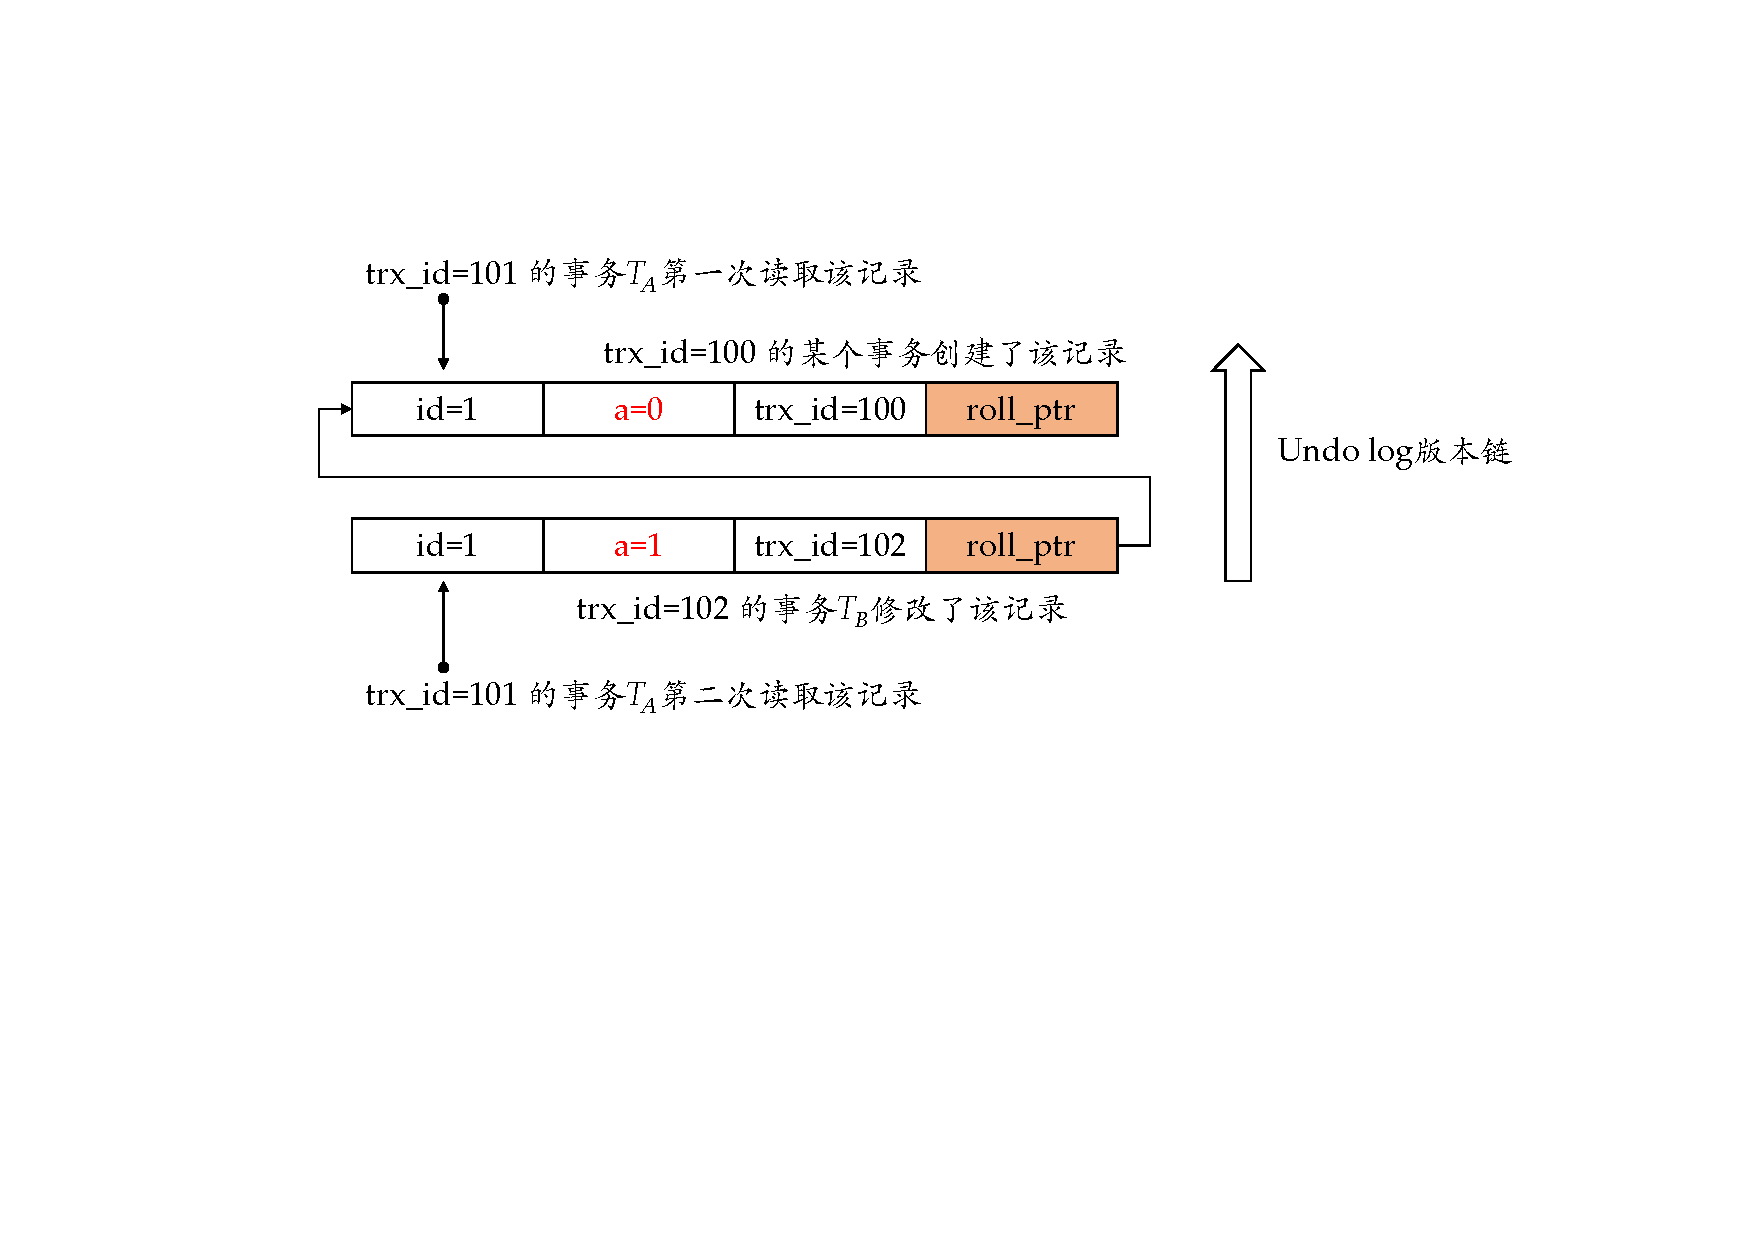
\includegraphics[width=.8\textwidth]{figure/MVCC-2.pdf}
    \caption{MVCC读取}
\end{figure}

现在我们首先假定: $T_A$处于read committed级别.

\begin{enumerate}
    \item $T_A$第一次读取时的read\_view:
    \begin{itemize}
      \item current\_trx\_id: 101
      \item alive\_trx\_list: [101, 102]
      \item min\_trx\_id: 101
      \item max\_trx\_id: 103
    \end{itemize}
    $T_B$此时尚未提交, 只有前一个记录: $\text{db\_trx\_id}(\text{record}_{\text{id}=1})<\text{min\_trx\_id}$, 从而它对$T_A$可见, 返回$a=0$.
    \item $T_A$第二次读取时的read\_view:
    \begin{itemize}
      \item current\_trx\_id: 101
      \item alive\_trx\_list: [101]
      \item min\_trx\_id: 101
      \item max\_trx\_id: 103
    \end{itemize}
    $T_B$此时已经提交, 此时有: $\text{min\_trx\_id}\leq \text{db\_trx\_id}(\text{record}_{\text{id}=1})<\text{max\_trx\_id}$, 而且很明显$T_B$已经不在活跃队列之中, 所以它对于$T_A$可见, 返回$a=1$.
\end{enumerate}

\textcolor{red}{read committed下事务每次读取都会生成新的read\_view.}

现在我们假设$T_A$处于repeatable read级别:
\begin{enumerate}
    \item $T_A$第一次读取时的read\_view:
    \begin{itemize}
      \item current\_trx\_id: 101
      \item alive\_trx\_list: [101, 102]
      \item min\_trx\_id: 101
      \item max\_trx\_id: 103
    \end{itemize}
    $T_B$此时尚未提交, 只有前一个记录: $\text{db\_trx\_id}(\text{record}_{\text{id}=1})<\text{min\_trx\_id}$, 从而它对$T_A$可见, 返回$a=0$.
    \item $T_A$第二次读取时的read\_view:
    \begin{itemize}
      \item current\_trx\_id: 101
      \item alive\_trx\_list: \textcolor{red}{[101, 102]}
      \item min\_trx\_id: 101
      \item max\_trx\_id: 103
    \end{itemize}
    $T_B$此时已经提交, 此时有: $\text{min\_trx\_id}\leq \text{db\_trx\_id}(\text{record}_{\text{id}=1})<\text{max\_trx\_id}$, 但是$T_B$还在活跃队列之中, 所以它对于$T_A$不可见, 继续沿着db\_roll\_ptr回溯其他版本.
\end{enumerate}

\textcolor{red}{repeatable read下事务的read\_view保持不变.}

\begin{itemize}
  \item \textcolor{red}{read committed的非一致性读总是读取被访问行的最新一份快照数据.}
  \item \textcolor{red}{repeatable read的非一致性读总是读取事务开始时的行数据版本.}
\end{itemize}

\textbf{MVCC不能解决幻读!!!}
